% Options for packages loaded elsewhere
\PassOptionsToPackage{unicode}{hyperref}
\PassOptionsToPackage{hyphens}{url}
%
\documentclass[
]{book}
\usepackage{amsmath,amssymb}
\usepackage{lmodern}
\usepackage{ifxetex,ifluatex}
\ifnum 0\ifxetex 1\fi\ifluatex 1\fi=0 % if pdftex
  \usepackage[T1]{fontenc}
  \usepackage[utf8]{inputenc}
  \usepackage{textcomp} % provide euro and other symbols
\else % if luatex or xetex
  \usepackage{unicode-math}
  \defaultfontfeatures{Scale=MatchLowercase}
  \defaultfontfeatures[\rmfamily]{Ligatures=TeX,Scale=1}
\fi
% Use upquote if available, for straight quotes in verbatim environments
\IfFileExists{upquote.sty}{\usepackage{upquote}}{}
\IfFileExists{microtype.sty}{% use microtype if available
  \usepackage[]{microtype}
  \UseMicrotypeSet[protrusion]{basicmath} % disable protrusion for tt fonts
}{}
\makeatletter
\@ifundefined{KOMAClassName}{% if non-KOMA class
  \IfFileExists{parskip.sty}{%
    \usepackage{parskip}
  }{% else
    \setlength{\parindent}{0pt}
    \setlength{\parskip}{6pt plus 2pt minus 1pt}}
}{% if KOMA class
  \KOMAoptions{parskip=half}}
\makeatother
\usepackage{xcolor}
\IfFileExists{xurl.sty}{\usepackage{xurl}}{} % add URL line breaks if available
\IfFileExists{bookmark.sty}{\usepackage{bookmark}}{\usepackage{hyperref}}
\hypersetup{
  pdftitle={Mozambique NAP Draft (Camila)},
  pdfauthor={Camila},
  hidelinks,
  pdfcreator={LaTeX via pandoc}}
\urlstyle{same} % disable monospaced font for URLs
\usepackage{longtable,booktabs,array}
\usepackage{calc} % for calculating minipage widths
% Correct order of tables after \paragraph or \subparagraph
\usepackage{etoolbox}
\makeatletter
\patchcmd\longtable{\par}{\if@noskipsec\mbox{}\fi\par}{}{}
\makeatother
% Allow footnotes in longtable head/foot
\IfFileExists{footnotehyper.sty}{\usepackage{footnotehyper}}{\usepackage{footnote}}
\makesavenoteenv{longtable}
\usepackage{graphicx}
\makeatletter
\def\maxwidth{\ifdim\Gin@nat@width>\linewidth\linewidth\else\Gin@nat@width\fi}
\def\maxheight{\ifdim\Gin@nat@height>\textheight\textheight\else\Gin@nat@height\fi}
\makeatother
% Scale images if necessary, so that they will not overflow the page
% margins by default, and it is still possible to overwrite the defaults
% using explicit options in \includegraphics[width, height, ...]{}
\setkeys{Gin}{width=\maxwidth,height=\maxheight,keepaspectratio}
% Set default figure placement to htbp
\makeatletter
\def\fps@figure{htbp}
\makeatother
\setlength{\emergencystretch}{3em} % prevent overfull lines
\providecommand{\tightlist}{%
  \setlength{\itemsep}{0pt}\setlength{\parskip}{0pt}}
\setcounter{secnumdepth}{5}
\usepackage{booktabs}
\usepackage{booktabs}
\usepackage{longtable}
\usepackage{array}
\usepackage{multirow}
\usepackage{wrapfig}
\usepackage{float}
\usepackage{colortbl}
\usepackage{pdflscape}
\usepackage{tabu}
\usepackage{threeparttable}
\usepackage{threeparttablex}
\usepackage[normalem]{ulem}
\usepackage{makecell}
\usepackage{xcolor}
\ifluatex
  \usepackage{selnolig}  % disable illegal ligatures
\fi
\usepackage[]{natbib}
\bibliographystyle{plainnat}

\title{Mozambique NAP Draft (Camila)}
\author{Camila}
\date{2021-09-06}

\begin{document}
\maketitle

{
\setcounter{tocdepth}{1}
\tableofcontents
}
\hypertarget{executive-summary}{%
\chapter{Executive Summary}\label{executive-summary}}

\hypertarget{introduction}{%
\chapter{Introduction}\label{introduction}}

\hypertarget{national-context}{%
\chapter{National Context}\label{national-context}}

\hypertarget{national-circumstances}{%
\section{National Circumstances}\label{national-circumstances}}

\textbf{\emph{(From Second National Communication Draft)}}

\hypertarget{geography}{%
\subsection{Geography}\label{geography}}

The Republic of Mozambique is situated in the southern hemisphere, on the south-eastern coast of the African continent, between latitudes 10º27'S and 26º52'S and meridians 30º12'E and 40º51'E. The country has an area of 801,590 km2 of dry land and about 13,000 km² of inland water. The eastern part of the country is bathed by the Indian Ocean, with a coastline of approximately 2,700 km. In its northern part, it is bordered by Tanzania; to the northwest by Zambia, Malawi and Lake Niassa; Zimbabwe, to the west; South Africa, to the southeast; and to the south, by E-Swatini (then Swaziland), on a terrestrial international boundary line approximately 4,330 km long. To the east, the country is bounded by the Indian Ocean and separated from Madagascar by the Mozambique Channel (Figure 1.1).

Administratively, the country is divided into 10 provinces. However, the municipality of Maputo city (the country's capital) has the status of a province, bringing the number to 11. The provinces are currently divided into 154 districts (26 more districts from the previous 128) which, in turn, are divided into 419 local administrative districts, called administrative posts. The latter are made up of 1,052 Localities, the lowest level of administrative configuration in the Mozambican State. To the subdivisions reported above are added 53 municipal authorities, of which 33 were created in 1998, another 10 in 2008 and another 10 in 2013.

There are numerous islands along the 2,700 km of coastline, including the Quirimbas archipelago in Cabo Delgado province, Ilha de Moçambique and the Goa and Sena islands in Nampula province, the Bazaruto archipelago in Inhambane, and the Inhaca, Portugueses and Xefina islands in Maputo province.

\emph{Figure 1.1: Map of Mozambique with international boundaries}

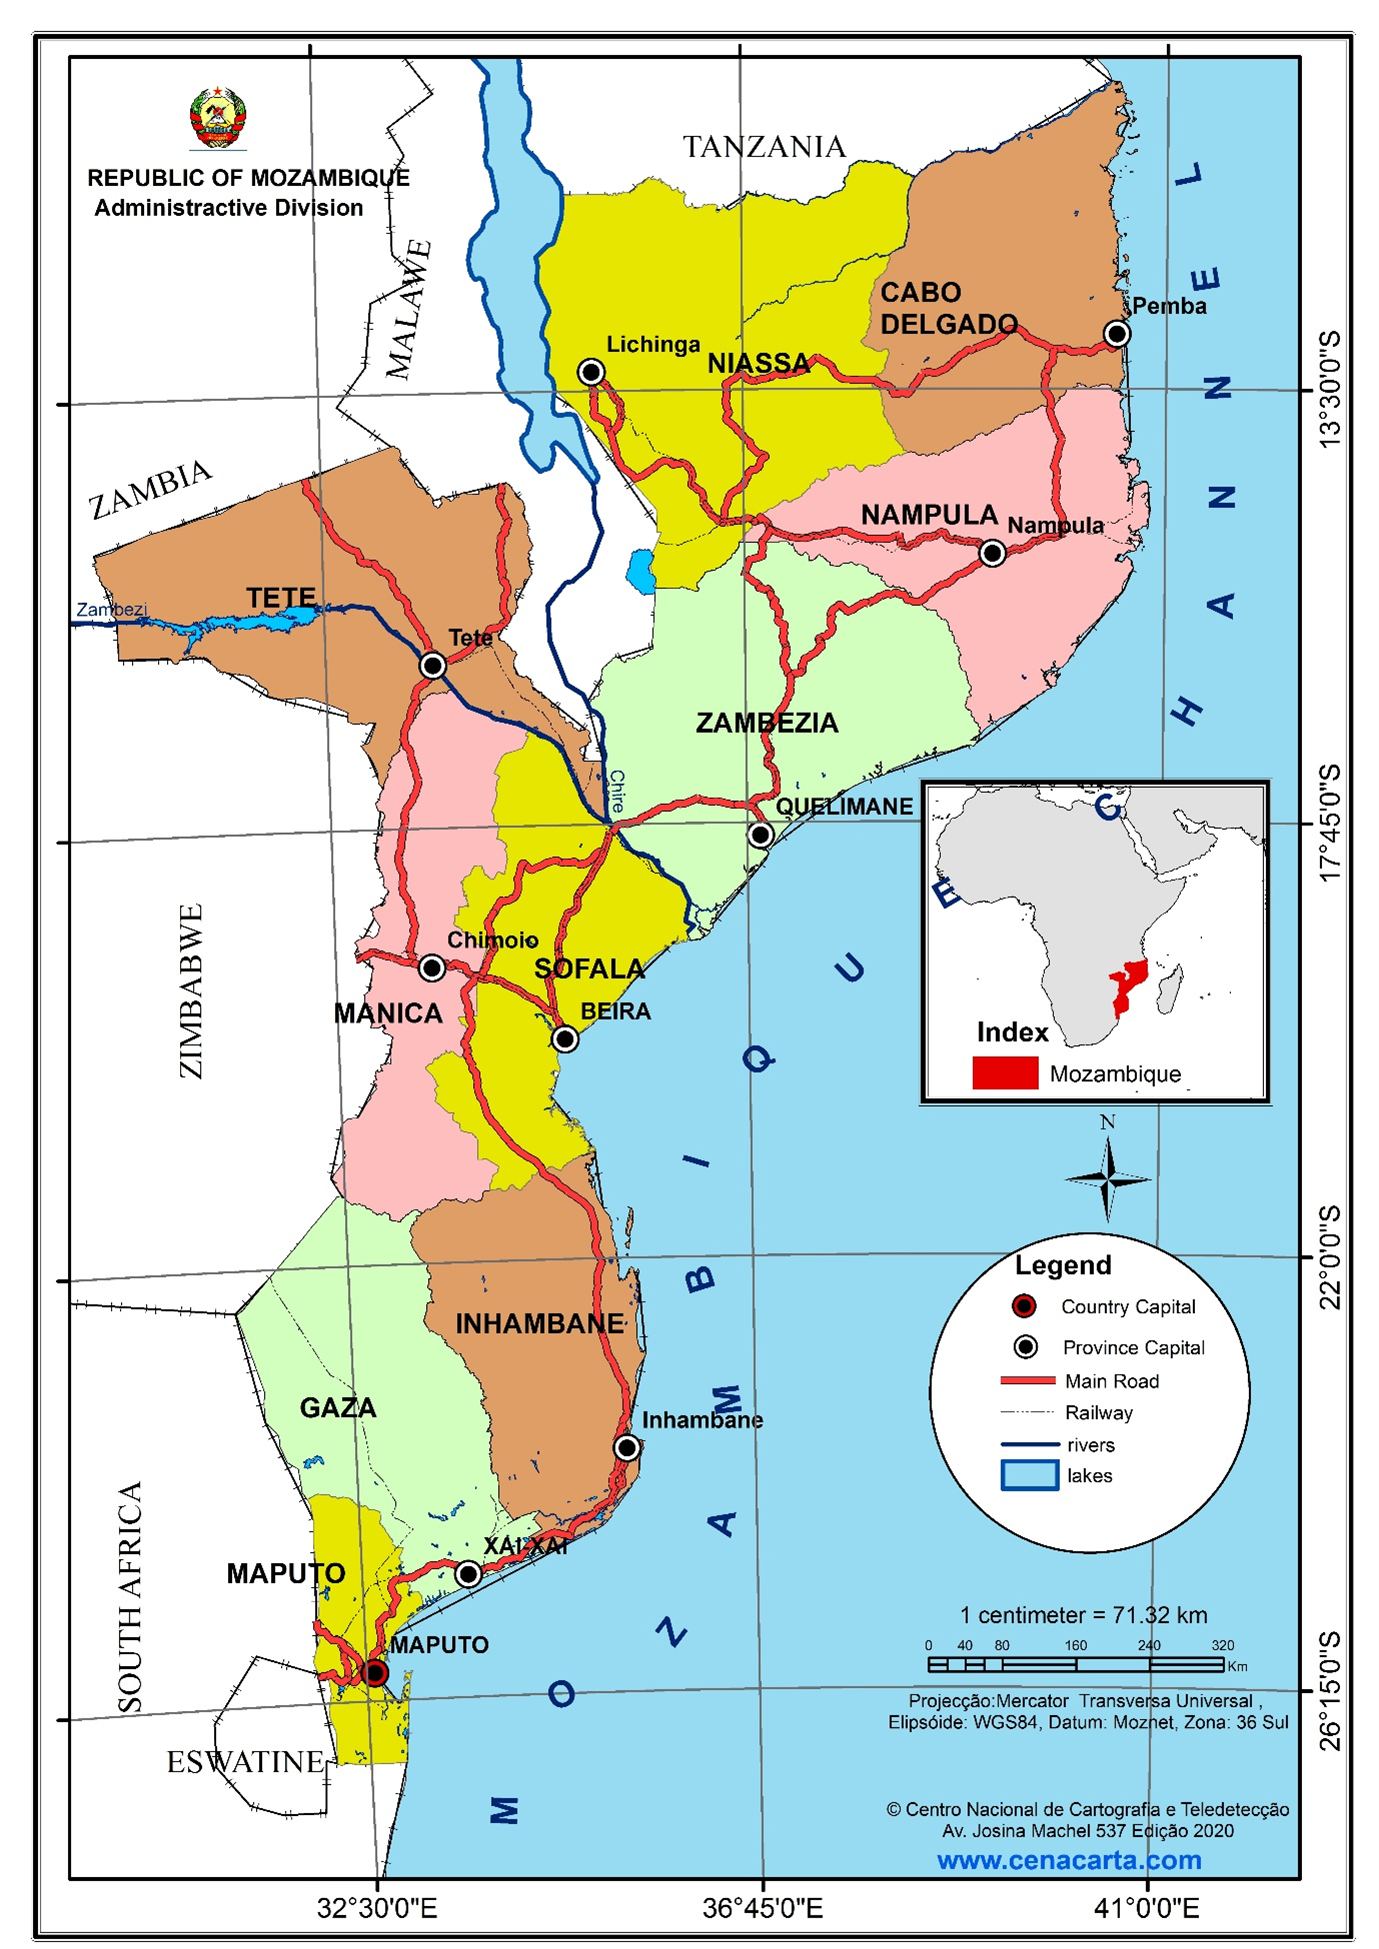
\includegraphics[width=0.9\textwidth,height=\textheight]{Picture1.png}

\emph{Figure 1.2: Map of geographical location of Mozambique with appropriate administrative division by provinces.}

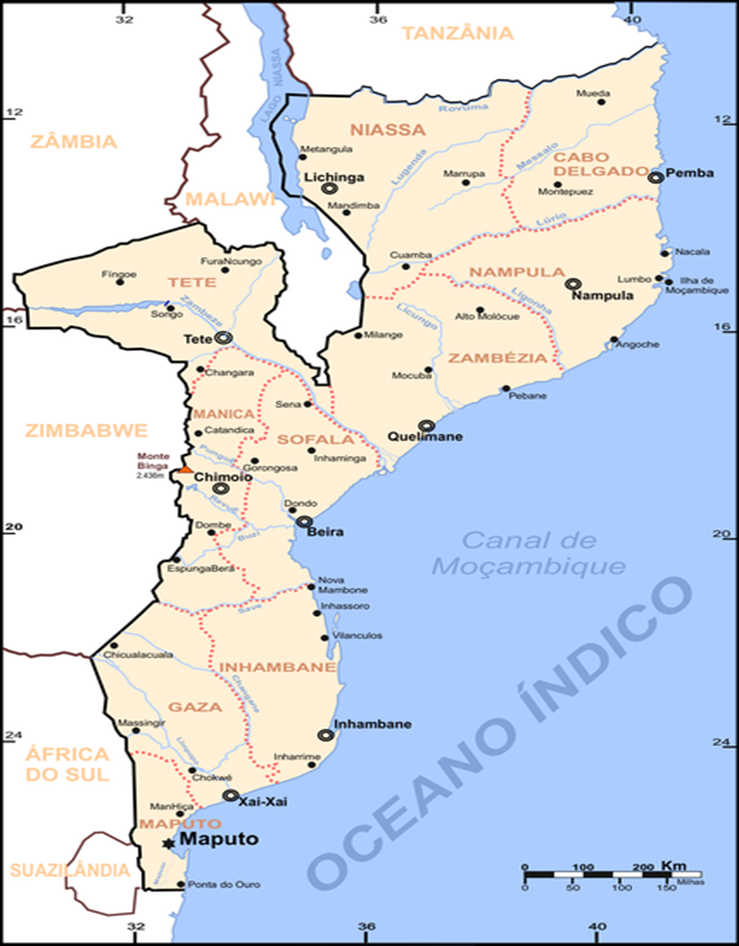
\includegraphics[width=0.85\textwidth,height=\textheight]{Picture2.png}

\hypertarget{population}{%
\subsection{Population}\label{population}}

The Mozambican population is 27,909,798 inhabitants (INE 2017), with about 52\% women and 48\% men. The distribution by age group is about 45\% for 0-14 years, 52\% for 15-64 years and 3\% for over 64 years (figure 1.3). The most widely spoken national languages in the country include KiSwahili, EMakhuwa, CiSena, XiNdau, XiTsonga, XiTchope, Guitonga, CiNyungwe, EChwabo, EKoti, ELomwe, CiNyanja, CiYao, XiMakonde and KiMwane, out of more than 40 languages in the country. The language adopted as official is Portuguese, inherited from the colonizing country, Portugal, from which Mozambique became independent on June 25, 1975.

Mozambique has registered significant population growth with an average annual rate of 2.4\% over the last ten years. Between 2007 and 2017 there was a growth of 8.4 million inhabitants, against 4.4 million between 1997 and 2007 (figure 1.3). According to projections, the Mozambican population may exceed 50 million inhabitants by 2050. These data show how the demographic issue will play a very important role in the planning of the country's socioeconomic development and the potential challenges for the management of natural resources that is the main source for the majority of the population, as well as the environment.

\emph{Figure 1.3: Population age structure (INE, 2017 census)}

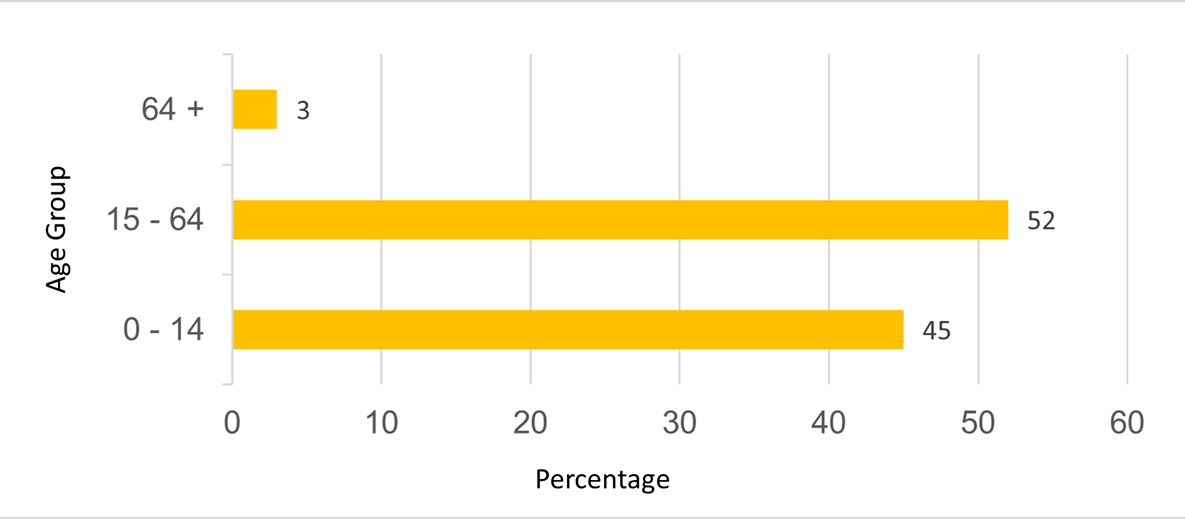
\includegraphics[width=0.9\textwidth,height=\textheight]{Picture3.png}

\emph{Source:} \url{http://www.ine.gov.mz/estatisticas/estatisticas-demograficas-e-indicadores-sociais/populacao}

Other demographic indicators are shown in Table 1.1. This table highlights the reduction in the maternal and infant mortality rate, as well as the increase in life expectancy. The illiteracy rate has also decreased, although it is still high, particularly among women.

\emph{Table 1.1: Evolution of demographic indicators in Mozambique between 1980 - 2017}


\includegraphics{Picture5.png}

\hypertarget{economy}{%
\subsection{Economy}\label{economy}}

Agriculture in Mozambique is the pillar of the national economy. The sector employs 90\% of the female labour force and 70\% of the male labour force, that is, 80\% of the Mozambican active population works in the agricultural sector (PEDSA, 2011). Agriculture has an average share in GDP above 20\% of the total. The trade and transport and communications services sectors contributed an average of 10\% each (Table 1.3). The extractive industry sector has shown great performance in recent years, rising from 2\% in 2013 to just over 7\% in 2018 (INE: National Accounts of Mozambique). The national economy has considerable potential in the primary sector, driven by the existence of natural resources, but the main challenge is the development of industries that allow for the sustainable exploration and transformation of these resources. Diversification of the national economy is still a challenge for more stable, comprehensive and sustainable growth. The Mozambican economy, after several years of growth of about 7\% per year, has slowed since 2016, due to various factors of international and national conjuncture (table 1.2).

\emph{Table 1.2: Evolution of Economic Indicators, 2008-2018}

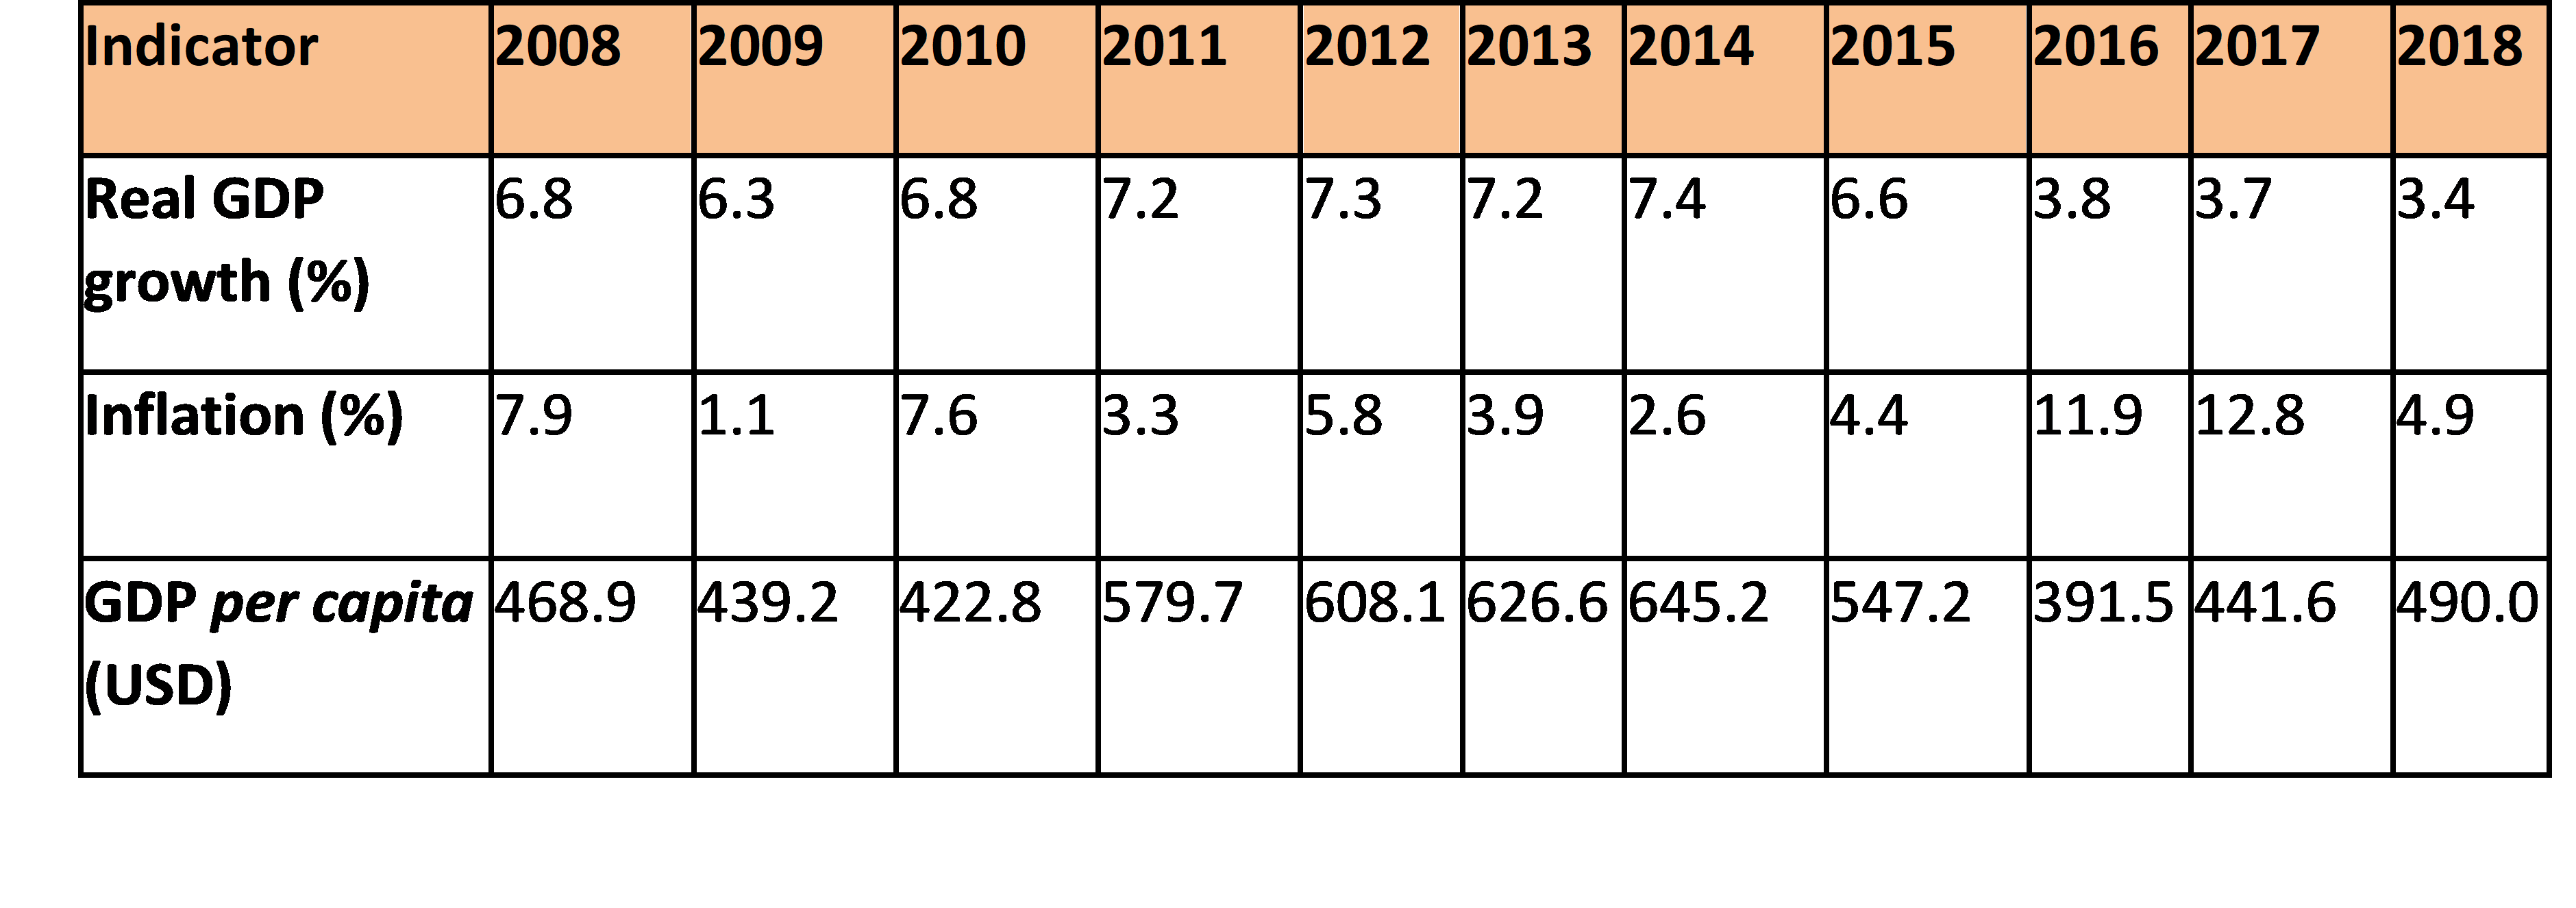
\includegraphics{Picture6.png}

\emph{Table 1.3: Contribution of sectors to GDP}

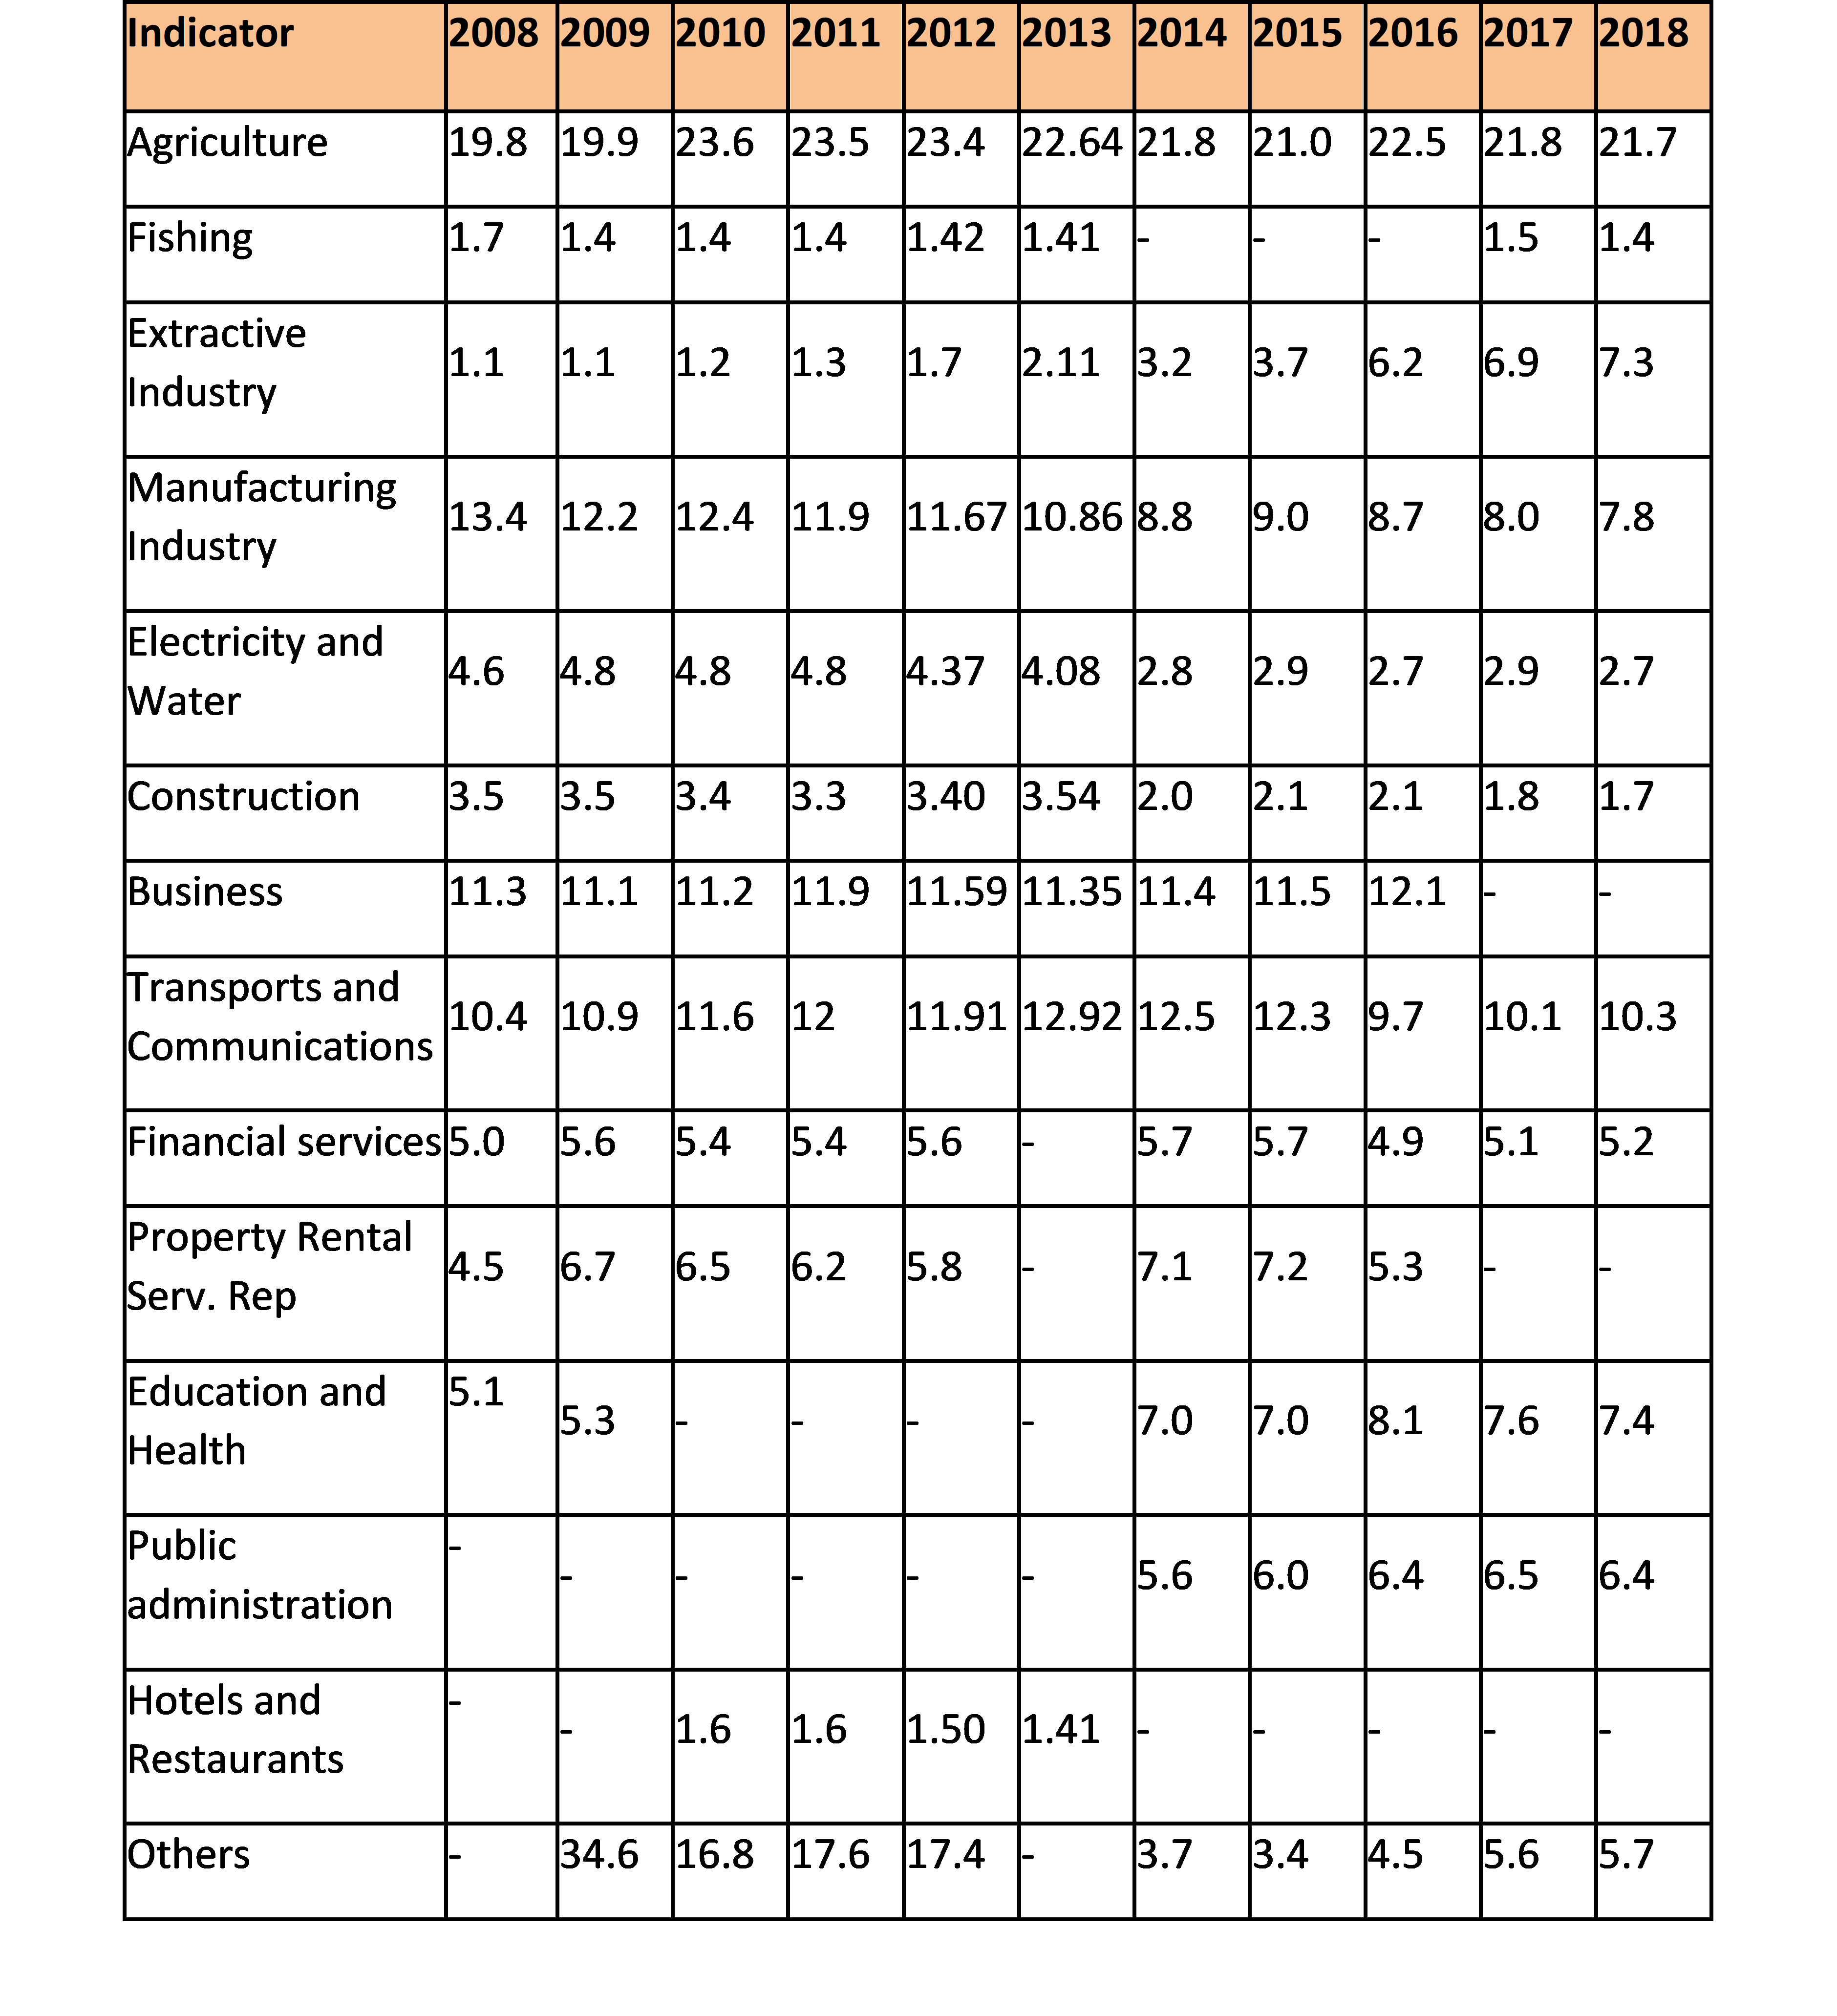
\includegraphics{Picture7.png}
\emph{Source: INE: National Accounts of Mozambique}

\hypertarget{relief}{%
\subsection{Relief}\label{relief}}

The relief of the country is arranged in the form of an amphitheater, with a mountainous area in the west, which descends in flattened steps to the coastal plain in the east. Thus, according to altitude, plains, plateaus, mountains and depressions are identified in Mozambique. The coastal plain, with altitudes of up to 200 meters, extends along the entire coastal strip, narrowing from the mouth of the Rovuma river to the Zambeze delta and extending southwards to the so-called great Mozambican plain, up to Ponta de Ouro. It occupies 1/3 of the national territory. There are also the so-called depression plains which extend along the valleys of the main rivers, eventually receiving the name of the respective hydrographic basins, for example: Incomati Plain, Limpopo Plain, Save Plain, Búzi Plain, Lúrio Plain, Lugela Plain, Messalo Plain and Zambezi Plain.

\includegraphics{Relief.png}

\begin{center}\rule{0.5\linewidth}{0.5pt}\end{center}

\textbf{\emph{(From General Outline Prototype NAP)}}

\hypertarget{geography-1}{%
\subsection{Geography}\label{geography-1}}

Mozambique is situated on the Eastern coast of Southern Africa, between 10º27´S and 26º52´S latitudes and 30º12´E and 40º51´E longitudes. The total land area is 784,090 Km². The country is divided into 11 provinces including Maputo city, which is also considered a province. About 70\% of the coutry is covered by savanna and secondary forests. Approximately 45\% of the territory has potential fos agriculture.

About 60\% of the land is classified as managed land, including agriculture and permanent pasture lands. The shelf area up to 200m depth and 104 Km² and the total area of the Exclusive Economic Zone is 562 Km².

The climate in the Northern region of the Zambezi River is under the influence of the equatorial low -- pressure zone with a NE monsoon in the warm season. The climate in the Southern area of Zambezi River is influenced by subtropical anti-cyclonic zone. In the North of Sofala, along the Zambezi River, lays a transitional zone with high rainfall figures.

In the North of Mozambique, the winds are influenced by the monsoon system with NE winds during the southern summer and SWwinds during the southern winter. Central and Southern Mpzambique are dominated by the SE trade winds.

The average annual precipitation is about 1200 mm. The rainfall is mainly restricted to the warm season, November to April. According to the classification of Köppen, the Norther areas ( Cabo Delgado, Niassa, Nampula and Zambezia) and the coastal region climate is classified as tropical rain savanna, whereas the climate of the upland areas of the interior is humid and temperate. Ocean currents, particularly the Mozambique warm current, may influence the rainfall.

Mozambique has more than 100 rivers. The major ones are: Rovuma, Lurio and Zambezi in North, Pungue, Buzi, Gorongosa and Save in the center and Limpopo, Incomati and Maputo in the South. These rivers drain about 208 Km3 of water rich in nutrients into the coastal waters. About 80\% of this water enters the ocean from Sofala Bank, central Mozambique. Zambezi River, the largest river in Eastern Africa, alone, contributes with 67\% of the total river discharge in the whole country.

The tidal rangr is about 2m in the South, 3.1m in the North and about 6.4m in the Center. High range in the center is throught to be related to both the shallowness and channel effects. The tidal wave entering the Mozambique Channel through the South would, due to Coriolis, induce an increment in the Mozambican coast.

In terms of administrative divisions and, in accordance with Mozambican Constitution, Mozambique is divided into eleven provinces, which are sub-diveded into 154 districts, Administrative Post and urban centres, which have also a special politicao-administrative status.

\emph{Source: Initial Communication 2003}

\hypertarget{institutional-arrangements}{%
\section{Institutional Arrangements}\label{institutional-arrangements}}

\hypertarget{legal-frameworks}{%
\section{Legal Frameworks}\label{legal-frameworks}}

\hypertarget{nap-info}{%
\chapter{NAP Info}\label{nap-info}}

\hypertarget{framework-for-the-nap}{%
\section{Framework for the NAP}\label{framework-for-the-nap}}

\hypertarget{essential-functions-of-the-nap-process}{%
\subsection{Essential functions of the NAP process}\label{essential-functions-of-the-nap-process}}

\hypertarget{the-nap-as-the-umbrella-programme-for-adaptation}{%
\subsection{The NAP as the umbrella programme for adaptation}\label{the-nap-as-the-umbrella-programme-for-adaptation}}

\hypertarget{coherence-with-national-development-context-sdgs-sendai-and-other-relevant-frameworks}{%
\subsection{Coherence with national development context, SDGs, Sendai and other relevant frameworks}\label{coherence-with-national-development-context-sdgs-sendai-and-other-relevant-frameworks}}

\hypertarget{nap-approach}{%
\section{NAP Approach}\label{nap-approach}}

\hypertarget{guiding-principles}{%
\subsection{Guiding principles}\label{guiding-principles}}

\hypertarget{a-systems-approach-to-adaptation}{%
\subsection{A systems approach to adaptation}\label{a-systems-approach-to-adaptation}}

\textbf{\emph{(From General Outline Prototype NAP)}}

The Government of Mozambique identifies climate shocks and seasonal variability, over exploitation of marine and timber resources, solid waste management, environmental sanitation and uncontrolled bush fires as major challenges.

\emph{Key economic sectors and systems}


\includegraphics{Systems.png}

\hypertarget{road-map}{%
\subsection{Road Map}\label{road-map}}

\textbf{\emph{(From General Outline Prototype NAP)}}

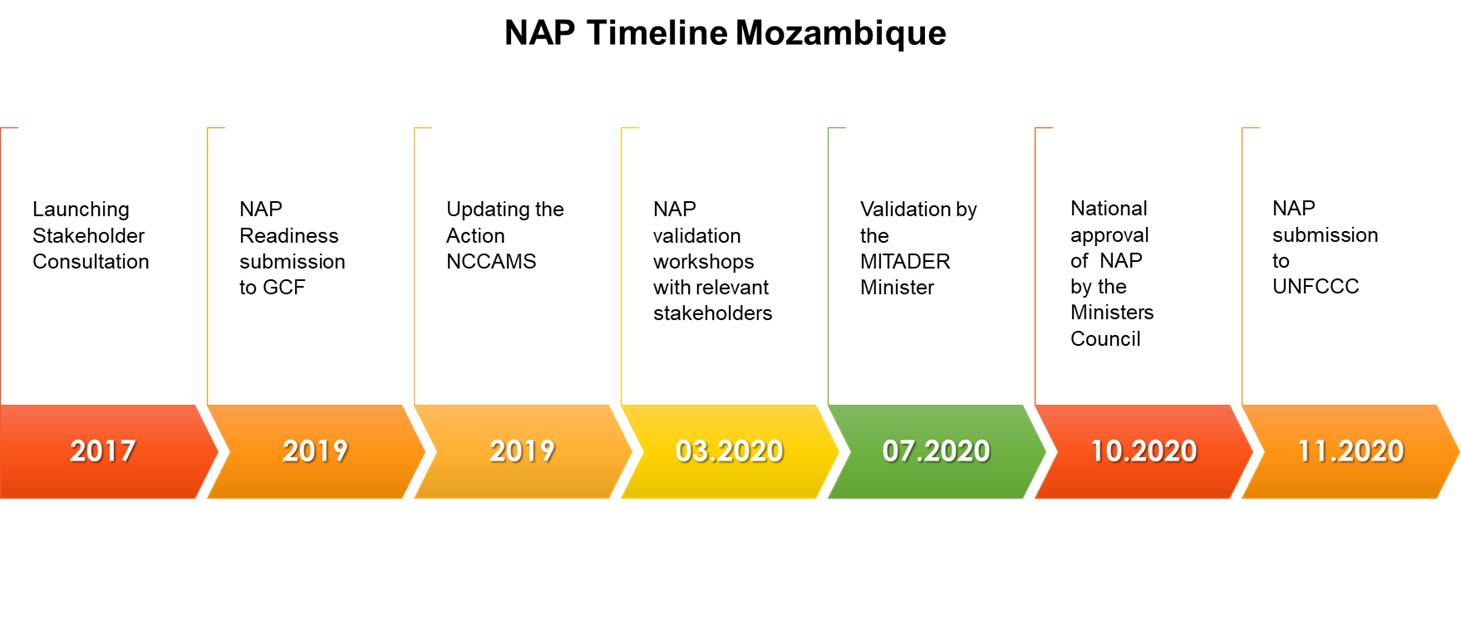
\includegraphics{Roadmap.png}

\hypertarget{vision-goals-and-objectives}{%
\section{Vision, goals and objectives}\label{vision-goals-and-objectives}}

\hypertarget{vulnerabilities-and-impacts-assessment}{%
\chapter{Vulnerabilities and Impacts Assessment}\label{vulnerabilities-and-impacts-assessment}}

\hypertarget{climate-analysis}{%
\section{Climate Analysis}\label{climate-analysis}}

\hypertarget{baseline-climate-based-on-1981-2010}{%
\subsection{Baseline climate based on 1981-2010}\label{baseline-climate-based-on-1981-2010}}

\begin{center}\rule{0.5\linewidth}{0.5pt}\end{center}

\textbf{\emph{(From Second National Communication Draft)}}

\textbf{Climate}

According to the Köppen-Geiger classification, the climate of Mozambique is generally of the Aw type (humid and dry tropical) and with pockets of BSh (hot semi-arid climate), with two very distinct seasons, one hot and rainy , from October to April, and the other cold and dry, from May to September (Gelcer et al.~2018). Other manifestations of climates of the As, Cfa and Cwa types can be found in isolation (figure 1.5).

\emph{Figure 1.5: Mozambican climate according to the Köppen-Geiger classification. As = tropical rainy climate; Aw = wet and dry tropical climate; BSh = hot semi-arid climate; Cfa = warm and humid temperate climate; Cwa = warm temperate climate with dry winter.}

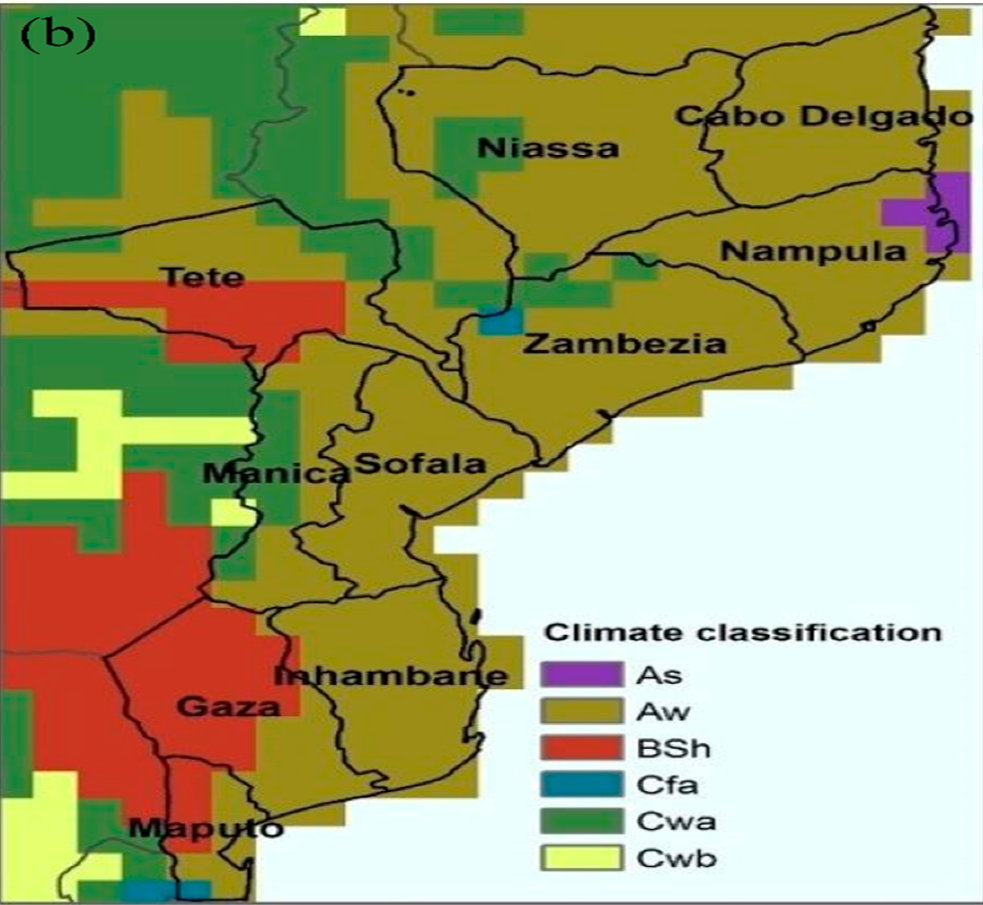
\includegraphics[width=0.85\textwidth,height=\textheight]{Climate-classification.png}

\emph{Source: Gelcer et al.~(2018).}

The atmospheric circulation in the country is characterized by zones of influence of low equatorial pressures with NE monsoon winds during the summer. The winds in the south and central zone are predominantly SE trades, and in the north zone they are influenced by a monsoon regime with NE winds during the summer and SW during the winter. Mozambique's precipitation regime is influenced by tropical cyclones formed in the southwestern Indian Ocean basin during the summer, the Intertropical Convergence Zone (ITCZ), the Indian Monsoon, the low pressure systems over the continent, Atlantic and Indian Anticyclones, El Niño/Southern Oscillation (ENOS) and Cold Fronts (Macie, 2016).

The spatial distribution of precipitation varies widely across the country. Precipitation is most abundant in the northern zone, where the annual average varies between 800 and 1,200 mm, becoming exceptionally high, 1,500 mm, in the highlands of Zambezia, Niassa and mountainous areas of Gorongosa. Central Mozambique and the entire coastline receive amounts of rain ranging between 800 and 1,000 mm. However, in some regions of the province of Tete, precipitation values can decrease by up to 600 mm. The south of the country is generally drier, with an average rainfall of less than 800 mm, reaching values of 300 mm at the administrative post of Pafuri, in Gaza province (figure 1.6).

\emph{Figure 1.6: Spatial distribution of accumulated annual precipitation in Mozambique}

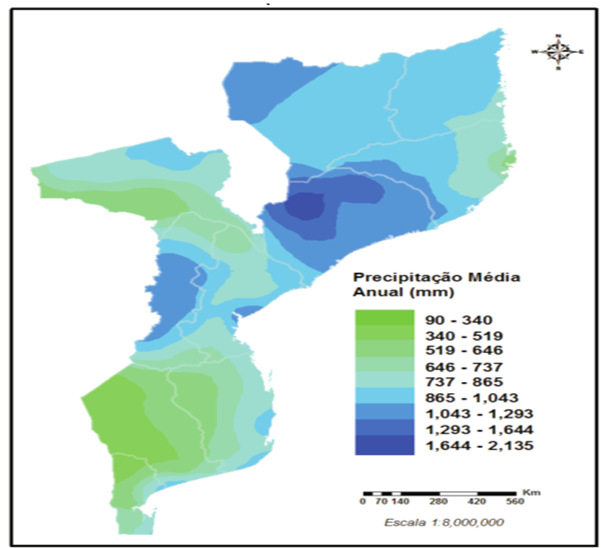
\includegraphics{Precipitation-distribution.png}

\emph{Source: Mozambique Precipitation Atlas, INAM, 2012}

\textbf{\emph{Seasonal Precipitation Variation}}

The period of greatest rainfall in the country corresponds to the summer in the Southern Hemisphere, between October and April. During the rainy season, the highest precipitation values occur in the months of January, February and March (figure 1.7), contributing to about 45\% of the total annual precipitation and is often associated with the migration and activity of the Inter-Tropical Convergence Zone (ITCZ).

In the northern region of the country, typical monthly precipitation values are 20 -- 200 mm/month during the rainy season and 5 -- 30 mm/month in the dry season. The central region registers between 30 -- 200 mm/month in the rainy season and 20 -- 40 mm/month in the dry season. Southern Mozambique, with the lowest precipitation values, registers between 40 -130 mm/month in the rainy season and 20 - 40 mm/month in the dry season. It is mainly the southern region that is prone to drought and some southern parts of Tete province in the center of the country.

\emph{Figure 1.7: Seasonal variation in monthly rainfall accumulated in different regions of the country}

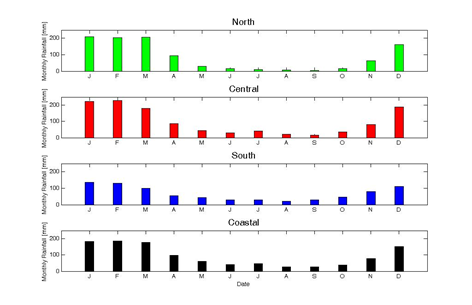
\includegraphics{Rainfall-variation.png}

\emph{Source: INGC, 2009}

\textbf{\emph{Interannual variation of precipitation}}

In Mozambique there is very high inter-annual rainfall variability in the rainy season, particularly in the central and southern regions. This variability causes significant fluctuations in the annual amounts of precipitation, with years with an abundance of precipitation (with greater probability of floods or inundation) or precipitation deficit (with greater probability of droughts) being registered. Figure 1.8 shows rainfall deviations from the climatological mean in four geographic regions of the country including the coastal region, from 1960 to 2006. The best-documented cause of this variability is the southern oscillation and the El Niño phenomenon (ENSO), which causes on average warmer and drier conditions; and relatively cooler and wetter conditions (La Niña) in the rainy season of eastern southern Africa. Evidence on the relationship between ENSO and rainfall in southern Africa can be found in several studies (Reason et al., 2000; Reason and Jagadheesha, 2005).

\emph{Figure 1.8: Precipitation deviations showing intra-annual variability and probability of occurrence of floods and droughts in four regions of the country, north, centre, south and coastal}

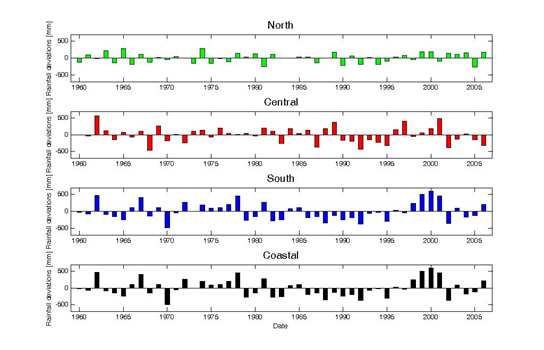
\includegraphics{Precipitation-variability.png}

\emph{Source: INGC, 2009.}

\textbf{Average Temperatures}

In general, average temperatures in Mozambique range between 25 -- 30 °C (average maximum temperatures) and between 15 -- 21 °C (average minimum temperatures) (figure 1.9). The highest mean maximum temperatures are recorded in the coastal area of the country, in the south of Tete province and in the western part of Gaza province (figure 1.9 on the left). As for the average minimum temperatures, these have a decreasing pattern from the coast to the interior. The highest average minimum temperatures are recorded along the northern coast, while the lowest are found in Gaza province (WFP, 2018). In this region of Gaza, there is also the largest temperature range in the country.

\emph{Figure 1.9: Spatial distribution of mean maximum temperature (left) and mean minimum temperature in Mozambique, calculated for the period 1982 - 2017.}

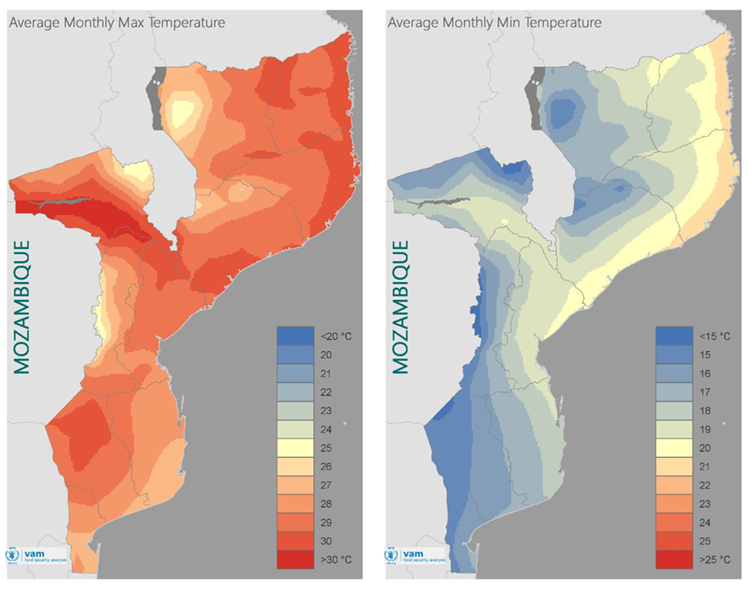
\includegraphics{Temperature-average.png}
\emph{Source: WFP, 2018. Mozambique Climate Analysis.}

\textbf{\emph{Historical Trends}}

Average temperature trends show positive variations (increase in average temperature) in most parts of the country. Studies indicate that the average annual temperature increased by 0.6 °C between 1960 -- 2006, at an average rate of 0.13 °C per decade for most seasons of the year (INGC, 2009). The study also points to an increase in the frequency of hot days and nights (days with a maximum temperature\textgreater{} 30 °C and nights with a minimum temperature\textgreater{} 20 °C respectively). The average number of ``hot'' days per year in Mozambique increased by 6.8\% of days (\textasciitilde25 days) and the average number of ``hot'' nights per year increased by 8.4\% of nights (\textasciitilde31 nights) during the same period in analysis (1960 and 2006).

\emph{Maximum and minimum temperatures}

Trends in increasing maximum and minimum temperatures (warming) have not been uniform across the country. Increases in mean maximum temperature of greater magnitude were recorded in the North (0.76 -- 1.16 °C), followed by central Mozambique between 1960 and 2006. Changes in average minimum temperatures in certain regions of the country are even greater, indicating large increases between 1.12 - 1.62°C (in the central region of the country) during the same period under analysis (INGC, 2009). Tables 1.4 and 1.5 provide a summary of trends in average maximum and minimum temperatures for different regions of the country.

\emph{Table 1.4: Change in mean maximum temperature (Tmax, °C) for each region between 1960 and 2006}

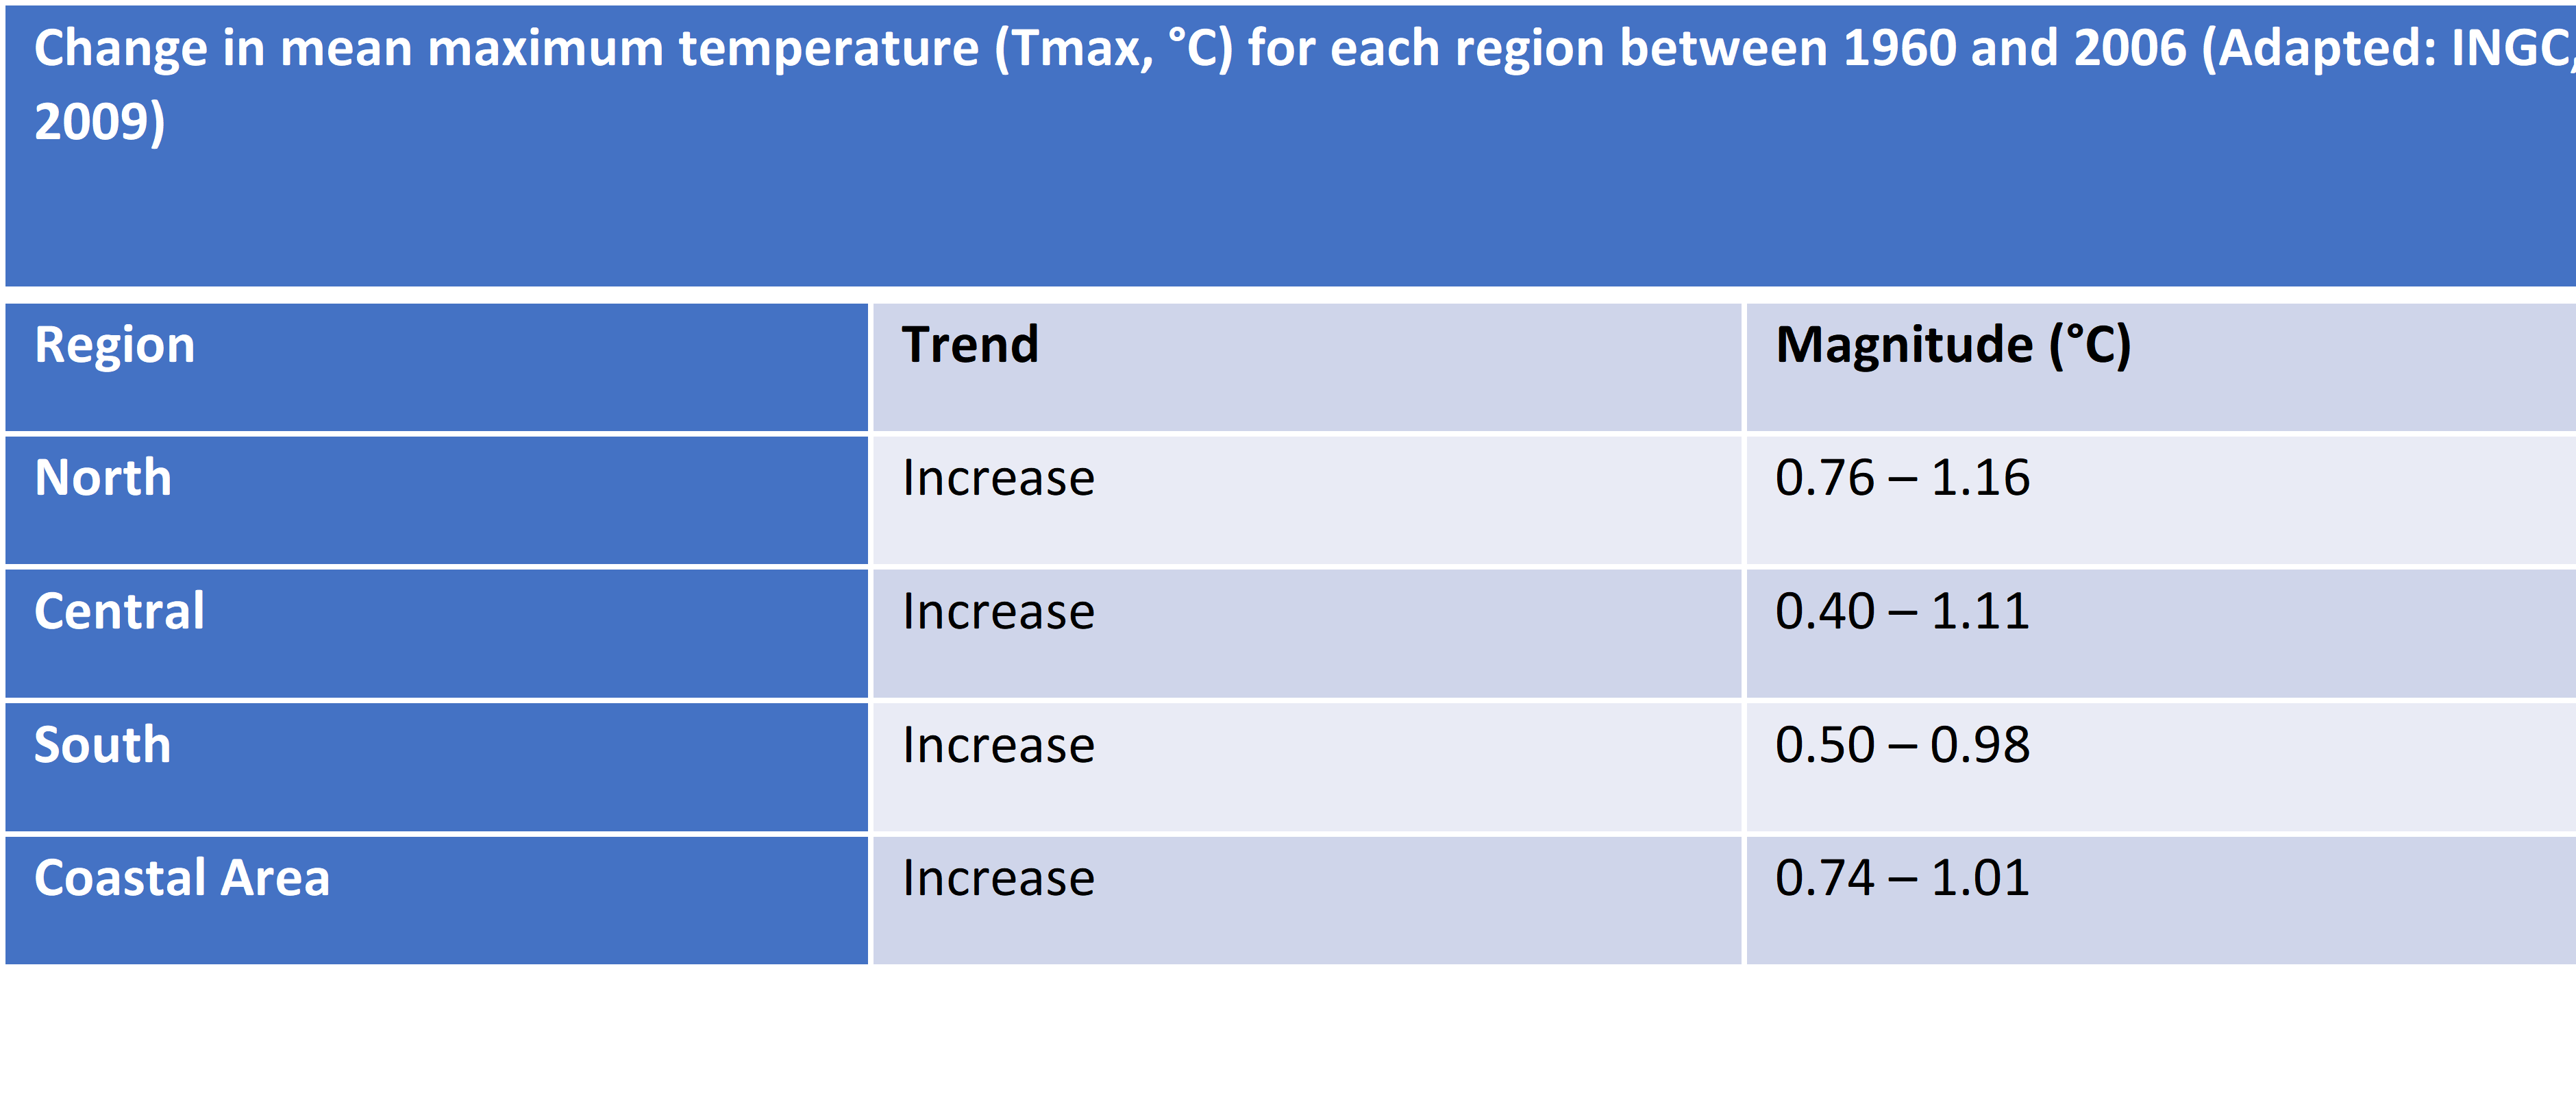
\includegraphics{Temperature-max.png}
\emph{Adapted: INGC, 2009}

\begin{center}\rule{0.5\linewidth}{0.5pt}\end{center}

\emph{Table 1.5: Change in mean minimum temperature (Tmin, °C) for each region between 1960 and 2006}

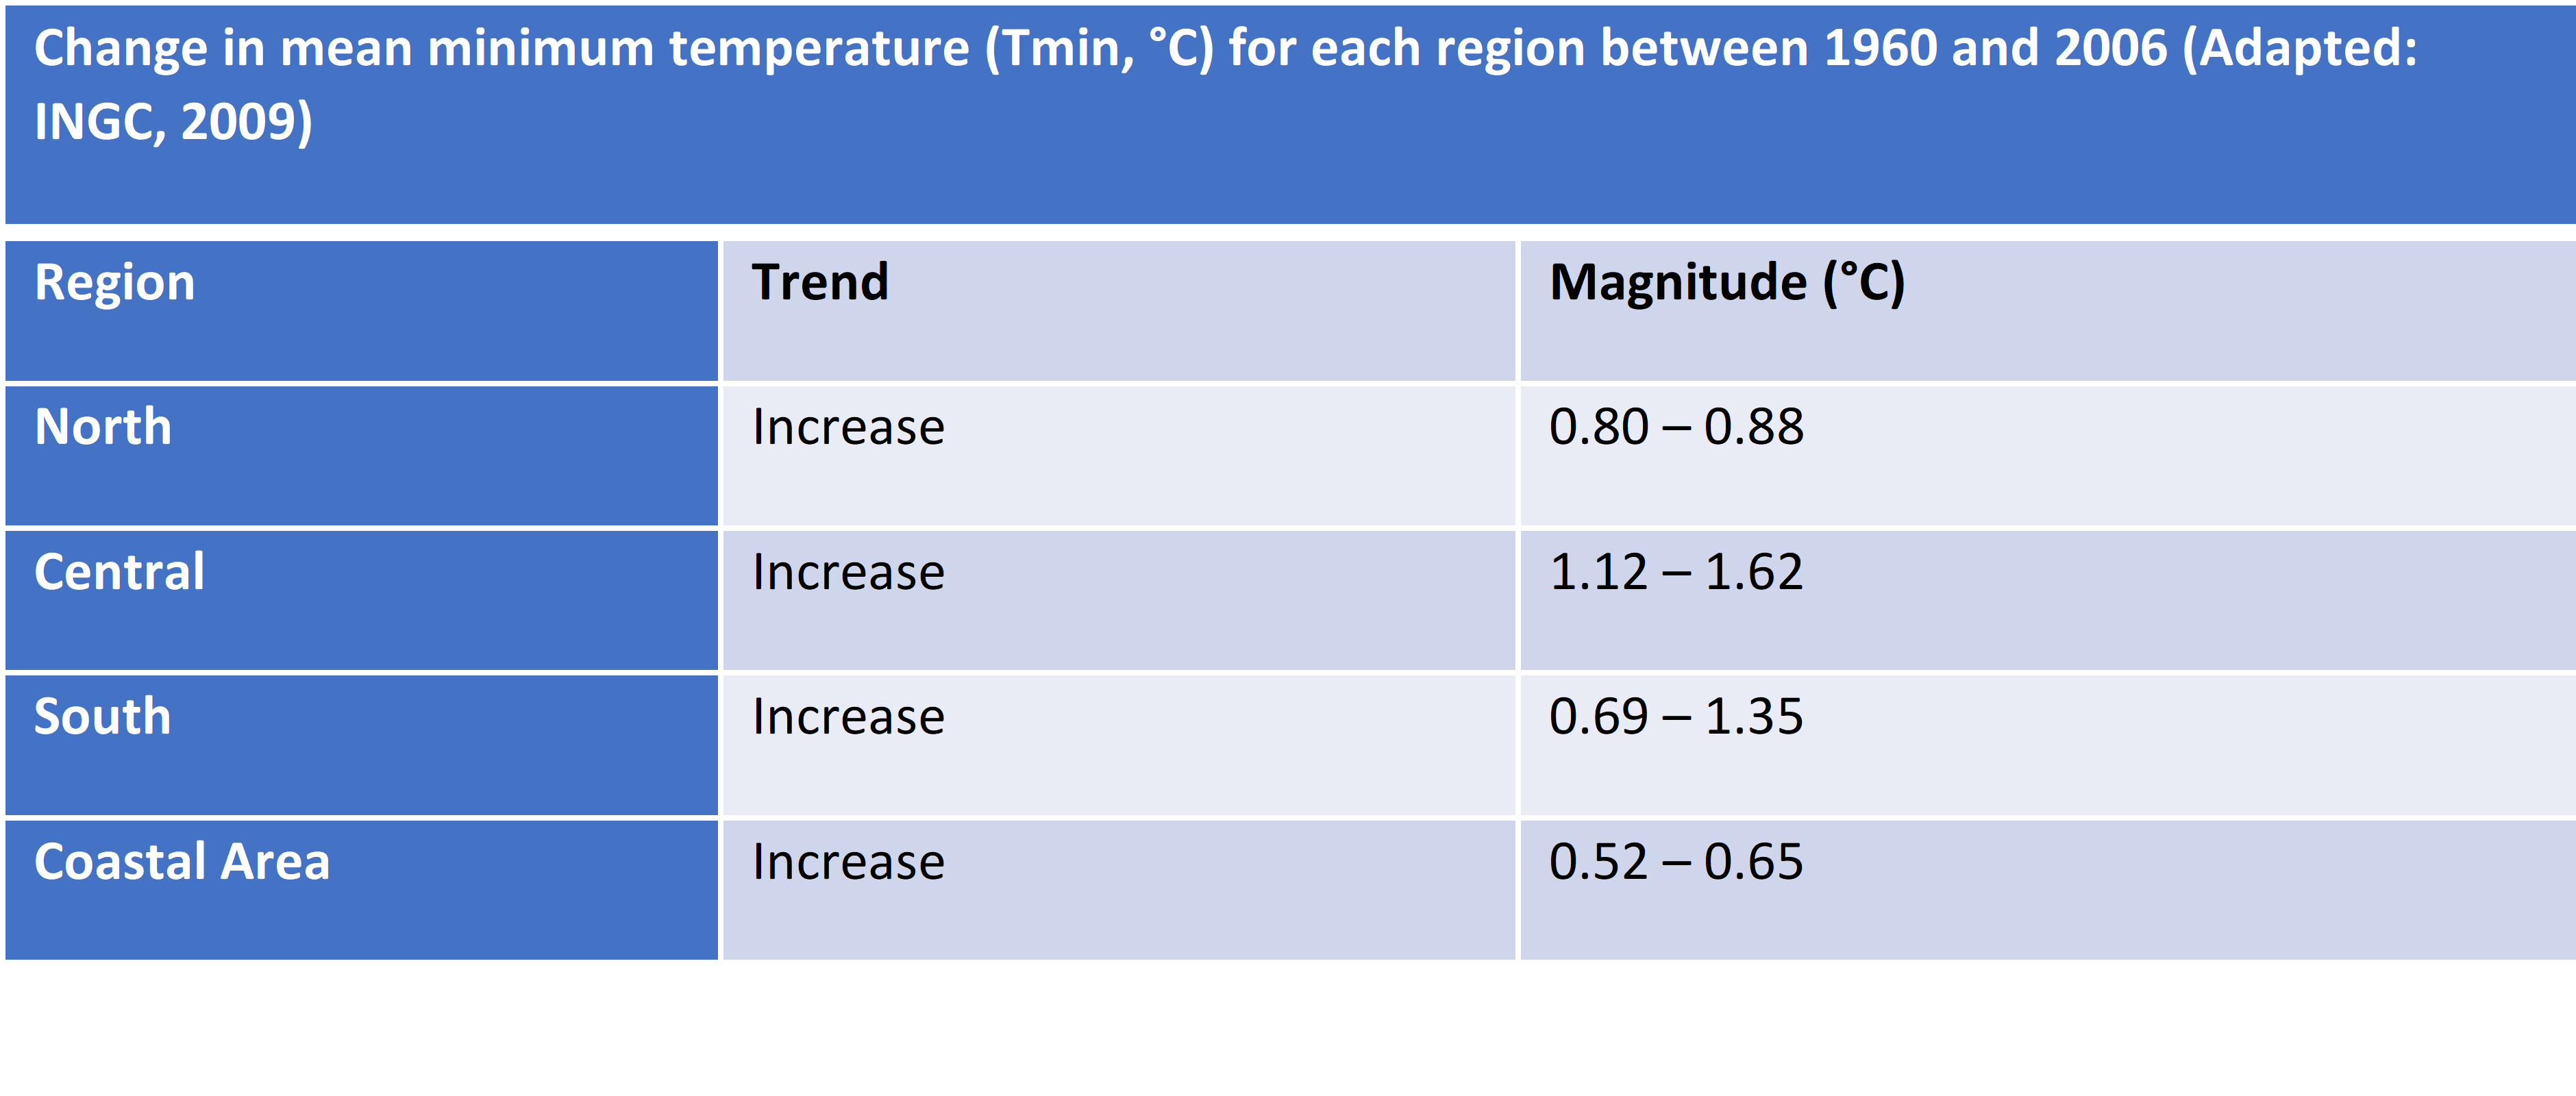
\includegraphics{Temperature-min.png}
\emph{Adapted: INGC, 2009}

\begin{center}\rule{0.5\linewidth}{0.5pt}\end{center}

\emph{Precipitation Trends}

Precipitation trends in the country are not significantly observable, due to the great inter-annual variability of rainfall in different seasons. However, the analysis of historical data made in several studies points to a late start of the rainy season in Mozambique, as well as an increase in the persistence of dry days.

The INGC report (2009), analysing data between 1960 and 2006, indicates a delay in the start of the rainy season that can reach between 20 and 45 days in some places, as well as a more pronounced persistence of dry days in the Northeast of the country from March to May and September to November.

The study by Mcsweeney et al.~(2010) found that in the period between 1960 and 2006, the average annual rainfall in Mozambique decreased at an average rate of 3.1\% per decade, in the period under review. On the other hand, despite the decreases observed in total rainfall, the amount of rain falling during heavy rain events increased at an average rate of 2.6\% per decade, with these increases being more pronounced in the period from December to February (DJF ).

\emph{Climate Projections}

\begin{itemize}
\tightlist
\item
  Future Temperature Projections
\end{itemize}

The Intergovernmental Panel on Climate Change (IPCC) in its Fifth Assessment Report (AR5) presents unequivocal evidence of climate change around the world: the atmosphere and oceans are warming, the extent and volume of snow and ice is decreasing, sea levels are rising and weather patterns are changing. The most optimistic scenario predicts an increase in the Earth's temperature between 0.3 °C and 1.7 °C and, in the worst case scenario, the Earth's surface could warm between 2.6 °C and 4.8 °C over this century by 2100 (IPCC, 2014) . The Paris Agreement approved in December 2015 under the United Nations Framework Convention on Climate Change (UNFCCC) established a global framework to reduce carbon dioxide (CO2) emissions and noted that global warming should be limited to 1.5°C.
In Mozambique, some studies point to a significant increase in temperature, with the average annual temperature projected to increase between 1.0 to 2.8 °C by 2060 and between 1.4 to 4.6 °C by 2090 (INGC, 2009; Mcsweeney et al.~al., 2010) (figure 1.10). The projected rate of warming will be faster in inland Mozambique than in areas closer to the coast. All projections indicate substantial increases in the frequency of days and nights considered ``hot'' in the current climate. This increase will be between 17 and 35\% of days per year around 2060, and between 20 and 53\% of days per year in 2090. The same projections also indicate a reduction in the frequency of days and nights considered ``cold'' in the current climate.

\emph{Figure 1.10: Average annual temperature trends in Mozambique between 1960 and 2006 (black line) and the projected future for three emission scenarios (colored lines). The colored bars on the right side indicate the different scenarios used in the simulations (A2, A1B and B1) as well as the uncertainty ranges in the average climate projections around 2090 -- 2100}

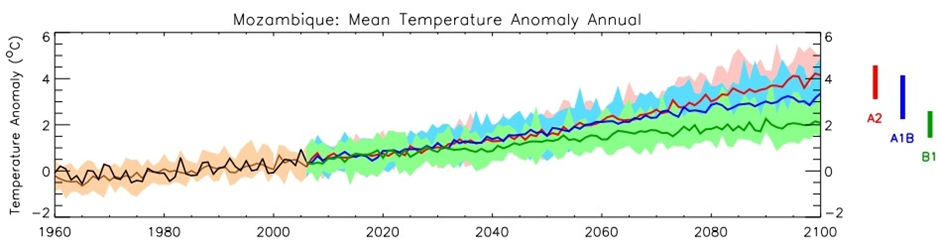
\includegraphics{Temperature-mean.png}
\emph{Adapted from Mcsweeney et al., 2010.}

\emph{Future Precipitation Projections}

Precipitation variations are not as clear as temperature variations. The range of precipitation projections resulting from different models is large and encompasses both negative and positive changes. There are indications of variations between -15 to +20 mm per month, or -15\% to +34\% (Mcsweeney et al., 2010). However, the models show more consistency in seasonal projections, indicating a reduction in rainfall in the dry season, that is, in the period from June to August (JJA) and from September to November (SON). This reduction is partially offset by increased rainfall in the rainy season, from December to February (DJF), with greater expression in northern Mozambique (Mcsweeney et al., 2010). In general, precipitation projections do not indicate substantial changes in annual precipitation, but rather changes in precipitation patterns (Figure 1.11).

\emph{Figure 1.11: Spatial patterns of monthly rainfall averages from September to November projected for the years 2030, 2060, and 2090}

\includegraphics{Rainfall-projections.png}
\emph{Adapted from Mcsweeney et al., 2010.}

\hypertarget{vulnerabilities-impacts-and-risks}{%
\section{Vulnerabilities, impacts and risks}\label{vulnerabilities-impacts-and-risks}}

\textbf{\emph{(From Second National Communication Draft)}}

\textbf{Introduction}

Mozambique is vulnerable to climate change due to its geographic location, low adaptive capacity as a result of poverty, limited investments in technology and weak infrastructure and social services. Climate change manifests through increased frequency and intensity of extreme events (droughts, floods, floods, event storms and tropical cyclones), rising sea levels, changes in temperature and precipitation patterns.

The consequences of the impacts of climate change include loss of human life, destruction of social and economic infrastructure, loss of domestic animals, loss of agricultural areas and crops, increased prices of agricultural products, deterioration of human health, environmental degradation with emphasis on erosion and saline intrusion.

This chapter presents the results of the vulnerability assessment and adaptation measures carried out in 2010, which covered the following sectors/areas: agriculture (maize cultivation in Chokwé); pastures and livestock, in the Limpopo basin; water resources, the Maputo basin was considered; fishing, shrimp in the Sofala bank; the coastal zone; mopane forests; and, health considered malaria and cholera. In the process of updating the SNA that started in 2020, other relevant sectors/areas were included, namely, biodiversity, infrastructure, energy and social protection, for which a review of the existing literature was carried out. Information on the impact of extreme events that occurred in the country in the sectors/areas covered was also included, using the Balance Sheet Reports of the Rainy Seasons produced by INGD.

Information on the vulnerability of the health sector was updated based on the preliminary results of the study ``Assessment of the Vulnerability and Adaptation to Climate Change of the Health Sector in Mozambique'' which includes the assessment of the impact of climate change on two climate-sensitive diseases in Mozambique: Malaria and Acute Diarrhea, carried out by MISAU.

In addition to the vulnerability assessment mentioned above, this chapter includes summary information on the vulnerability of 98 districts (Table 3.2) in which Local Adaptation Plans (PLAs) were formulated and approved within the scope of the implementation of ENAMMC. For the formulation of the PLAs in the districts, at least two communities in the district that participate in the assessment of the climate vulnerability and adaptability of the communities are involved -- Step 2 of the guide for the Formulation of Local Adaptation Plans. After the assessment with the communities, step 3 is followed, which is an assessment in the district. These two steps aim to determine the extent to which communities/districts are vulnerable to climate change, analysing trends, threats, opportunities and adaptive capacity of communities/districts to climate change and determining adaptation measures to improve their resilience to climate change.

The Guide for Formulating Local Adaptation Plans includes the Climate Vulnerability and Capabilities Analysis (CVCA) tools - developed by CARE and the Theory of Change (ToM). The PLAs are part of the short-term objectives defined by ENAMMC - increasing local resilience, fighting poverty and identifying opportunities for adaptation and low-carbon development at the community level, to be included in district planning.

\textbf{Climate Change Impacts}

\textbf{\emph{Disasters}}

Historical data on extreme events show that three climate-related hazards are most likely to occur in Mozambique, namely tropical cyclones, floods and droughts. These events are often associated with socio-economic damage, translated into loss of human life, human suffering, loss of assets, destruction of critical infrastructure (eg health facilities, schools, access roads, etc.) and other indirect losses.

An analysis of data from 1980 to 2019 shows that Mozambique was affected by 21 tropical cyclones, 20 flood events and 12 droughts (figure 3.1). This means that on average, the country is affected by a tropical cyclone or a flood event every two years and a drought event every three years. Tropical cyclones and flood events represent about 77\% of the total events that occurred in the period under review.

\emph{Figure 3.1: Total number of extreme events that occurred in Mozambique between 1980 -- 2019 }

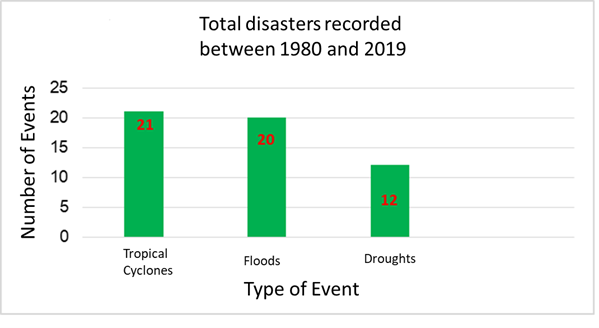
\includegraphics{Disasters.png}

\emph{Source: produced based on DeSinventar data and INGC rainy season balance reports.}

\textbf{\emph{Historical trends of extreme events}}

One of the crucial questions today is whether there is any evidence of an increase in extreme disaster-causing events or not. Through an analysis of the trend of events registered in the last four decades (1980 -- 2019), it is noted that the number of events that devastated the country increased significantly since the 2000s (figure 3.2). From the decade (2000-2010) to the current, the number of cyclones competes with the number of flood events, despite the slowdown of drought events.

Taking into account that tropical cyclones are often associated with heavy rain events that can contribute a significant proportion of precipitation in a very short period which in turn cause flooding in various regions of the country, with serious implications for the health of communities, the worsening of these phenomena in recent decades should deserve special attention from health authorities and beyond.

\emph{Figure 3.2: Trend in the number of extreme events occurring between 1980 and 2019.}

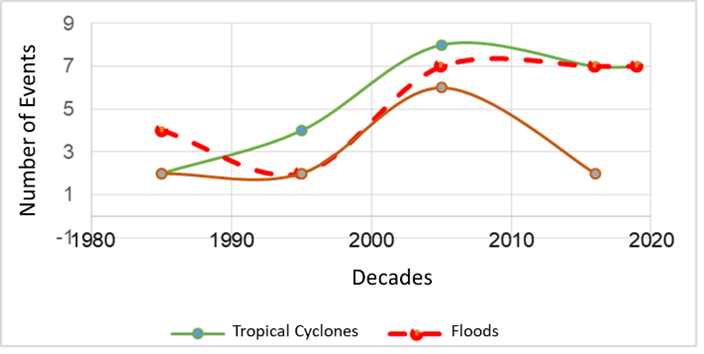
\includegraphics{Extreme-trends.png}

The direct impact of these events is often expressed by the number of human lives lost, people affected through loss of personal property and livelihoods, destruction of the country's critical infrastructure such as roads, bridges, water supply system, schools, hospitals, as well as the outbreak of water-borne diseases (e.g.~malaria, cholera, diarrhoea, etc.). However, the lack of systematic and homogeneous recording of events and their impacts and, on the one hand, the persistence in considering only large-scale and high-impact disasters over a short period of time have hidden thousands of small and medium-scale disasters that occur every year in the country. Consequently, Mozambique does not know the real value of direct and/or indirect economic losses associated with these events.

Table 3.1 presents the impact of climate change on the human dimension. Regarding the economic impacts, these are presented in the respective sectors where the vulnerability analysis is carried out.

\emph{Table 3.1: Summary of impacts of extreme events on the human dimension}

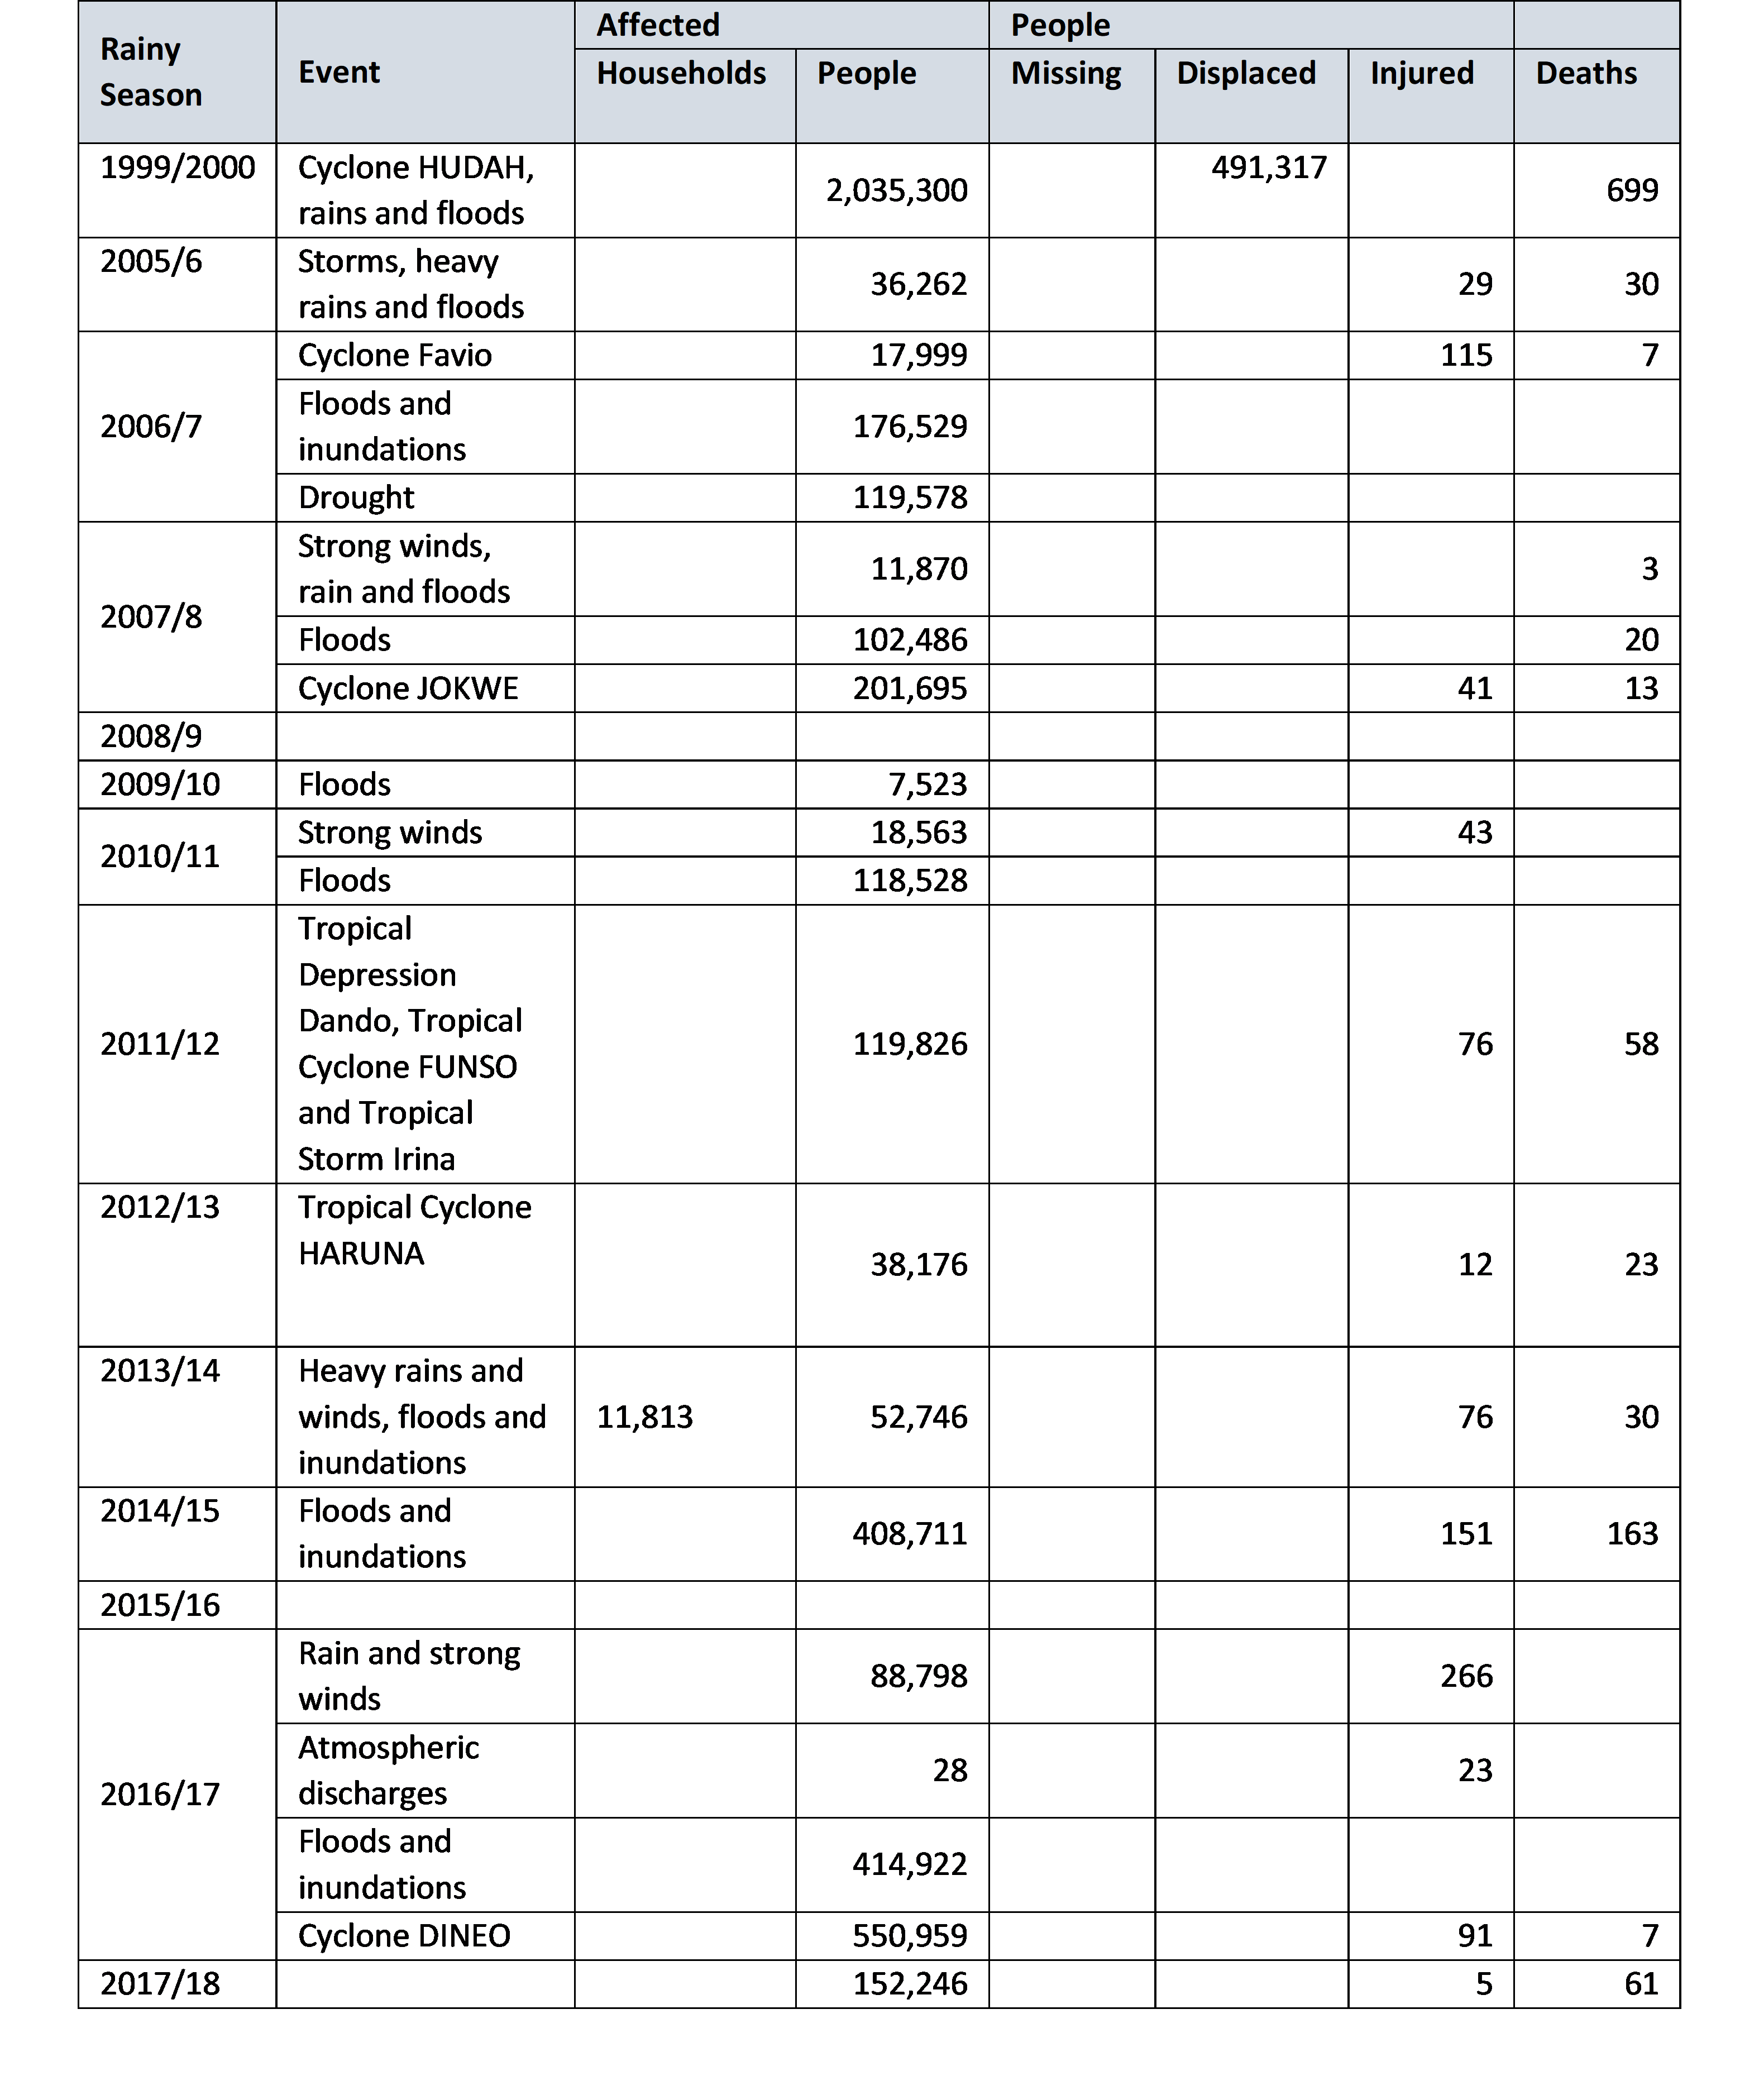
\includegraphics{Extreme-human.png}

\emph{Source: Rainy Season Balance Reports 2000, 2005/6 to 2017/18}

The extreme weather events that occurred in Mozambique in 2000 and in the rainy seasons from 2005/6 to 2017/18 affected an estimated 4,074,606 people, injured 885 people and caused 1,114 deaths. About 50\% of affected, injured and deaths resulted from the occurrence of Cyclone HUDAH, and it should be noted that tropical cyclones are events that cause greater impacts on the human dimension.

These impacts represent a setback in the process of poverty reduction, which is the priority of the Governments of developing countries, and increase their dependence on international aid. In this context, assessing the vulnerability of the most important social and economic sectors and identifying adaptation measures is of high priority.

\emph{Table 3.2: PLAs prepared in the period 2014 to 2018}


\includegraphics{PLAs.png}

The main threats indicated by communities and districts are grouped into droughts, floods and inundations, tropical cyclones/strong winds, sea level rise, epidemics, heat waves and/or cold spells, food insecurity, wildlife conflict and pests. (Include graph showing how each of the threats)

In addition to the PLAs, sector plans and other relevant instruments were also formulated, highlighting:

\begin{itemize}
\item
  The national action plan for the expansion of climate-resilient agriculture. This plan seeks to strengthen agricultural extension services to small farmers as well as knowledge management and sharing and strengthening in coordination with research and extension services;
\item
  Ministerial approval of national climate-resilient road standards and maintenance approaches; and the ministerial approval of mandatory climate risk screening for new road investments;
\item
  National Program for Productive Social Action (PNASP) through which households living in vulnerable districts are involved in public works activities in order to diversify their sources of income and, consequently, make them resilient.
\end{itemize}

\textbf{\emph{Climate Scenarios}}

The vulnerability analysis carried out at the SNC considered the climate projections developed by INGC ``Studies on the Impacts of Climate Change on Disaster Risk in Mozambique Synthesis Report -- Second Version'' in 2009.

The methodology of the INGC study was based on climatological modeling (temperature and rainfall) with the main purpose of understanding how Mozambique's climate may already be changing and how it can be expected to change in the future. This study details the observed changes in the country's seasonal climate during the period 1960 to 2005, in terms of temperatures and rainfall patterns (INGC, 2009).

Both historical trends and future projections were derived from daily temperatures (maximum and minimum) and rainfall values recorded since 1960, from 32 synoptic weather stations within Mozambique (INGC, 2009).

To project future scenarios in terms of the country's climate (temperature and rainfall), focusing on the mid-century (2046-2065) and late-century (2080-2100) periods, seven general circulation models were used: ECHAM, GFDL , IPSL, CCCMA, CNRM, CSIRO and GISS.

INGC's projections (2009) anticipate that climate change in Mozambique is mainly manifested in the following:

\emph{Temperature patterns}

\begin{itemize}
\item
  Atmosphere -- with an average increase between 1.5ºC and 3.0ºC in the period between 2046 and 2065 and recording of more hot days and fewer cold days, with an increase in the maximum and minimum temperature;
\item
  Oceans -- with rising mean sea levels and changes in the distribution and availability of fish stocks and effects on marine ecosystems (such as corals);
\end{itemize}

\emph{Precipitation patterns}

\begin{itemize}
\item
  With irregular rainfall behavior in terms of start and end times, rainfall (heavy precipitation phenomena in a short space of time) and duration of the rainy season (drought), disfiguring the notions of ``official'' and ``real'' start of the agricultural season, which may result in some regions in a decrease in current potential yields of around 25\%;
\item
  With a growing reduction in potential agricultural income levels of up to 20\% in the main crops that constitute the basis of food security and an essential condition for improving the per capita income of Mozambican families;
\end{itemize}

\emph{Increased frequency and intensity of extreme events (droughts, floods and tropical cyclones)}

\begin{itemize}
\item
  Persistence of the situation of extraordinary floods in identifiable places in the country which can be referred to as ``risk zones'';
\item
  Cyclones and other strong winds;
\item
  Prolonged droughts;
\end{itemize}

\emph{Sea level rise:}
15 cm, 30 cm and 45 cm as a consequence of thermal expansion and 15 cm, 110 cm and 415 cm as a consequence of the reduction of continental ice caps in the years 2030, 2060 and 2100, respectively;

\begin{itemize}
\item
  Areas with potential increased risk identified due to the emergence of other adverse natural phenomena such as loss by submersion and erosion of coastal areas, intrusion of saline water, desertification;
\item
  Reduction of areas available for agricultural practice in green or low-lying areas;
\item
  Many of the country's main coastal urban centers, including Maputo, Beira and Quelimane, are already in a critical situation in terms of vulnerability (human lives, properties, social infrastructure, etc.) to the effects of climate change.
\end{itemize}

\begin{center}\rule{0.5\linewidth}{0.5pt}\end{center}

\textbf{\emph{(General Outline Prototype NA)}}

Climate change impacts: highlights of recent impacts:

\begin{itemize}
\item
  Mozambique is particularly vulnerable to Climate Change (CC) due to its location downstream of shared watersheds (Floods, e.g.~2000 and 2013 Limpopo Basin; 2007 Zambeze, 2013 and 2019 Licungo Basin, etc.)
\item
  Increase in the frequency and intensity of extreme climatic events, such as droughts, floods and tropical cyclones (recent cyclones with high impact: Idai and Keneth 2019, Eline in 2000, etc.)
\item
  The long shoreline and the existence of extensive low-lands below sea level (sea level rise, storm surge, salt intrusion);.
\item
  The country's vulnerability is also increased by its low adaptive capacity, poverty, limited investment in modern technology, and weaknesses in its infrastructure and social services, especially those related to health and sanitation (e.g.~the malaria and cholera in 2019 after the cyclone Idai and Keneth in central and northern Mozambique).
\item
  These events result in the loss of human lives, crops, livestock and wildlife; the destruction of social and economic infrastructure; increased dependency on international support; food price increases; harm to human health and the environment; and the destruction of ecosystems.
\item
  CC represents a major barrier to the Government and its partners' efforts to fight poverty and achieve the MDGs.
  (Government of Mozambique, 2012)
\end{itemize}

\hypertarget{climate-change-adaptation-assessment}{%
\section{Climate Change Adaptation Assessment}\label{climate-change-adaptation-assessment}}

\hypertarget{priority-sectors}{%
\chapter{Priority Sectors}\label{priority-sectors}}

\hypertarget{agriculture}{%
\section{Agriculture}\label{agriculture}}

\textbf{\emph{(From Second National Communication Draft)}}

Agriculture is considered to be the basis for Mozambique's development. This sector is made up of small, medium and large producers. The most predominant class is smallholders who use approximately 97\% of the approximately five million arable land currently used for agriculture (Mozambique Government - PAPA, 2008).

In 2010, agriculture contributed 23\% to the Gross Domestic Product (INE). Furthermore, 80\% of the country's active population is employed in the agrarian sector. Thus, this sector is fundamental for poverty reduction and income generation for rural families, since most of this population depends on agriculture for food, employment and income.

A critical factor in agricultural production is access to and distribution of water throughout the vegetative cycle of crops. Production and productivity levels are affected by changes in climatic parameters, in particular variations in rainfall, given that around 98\% of farmers practice rainfed agriculture (CAP, 1999-2000).

According to the rainy season balance sheets, the agriculture sector is vulnerable to drought and drought events, floods and inundations, strong winds, tropical cyclones including pests (see Table 3.3). These events result in crop areas affected and/or lost; death and/or disappearance of domestic animals, especially cattle, goats, pigs, sheep and poultry; destruction of agricultural and animal management infrastructures; loss of pasture areas, affecting farmers and their families.

\emph{Table 3.3: Impact of climate change on agriculture}

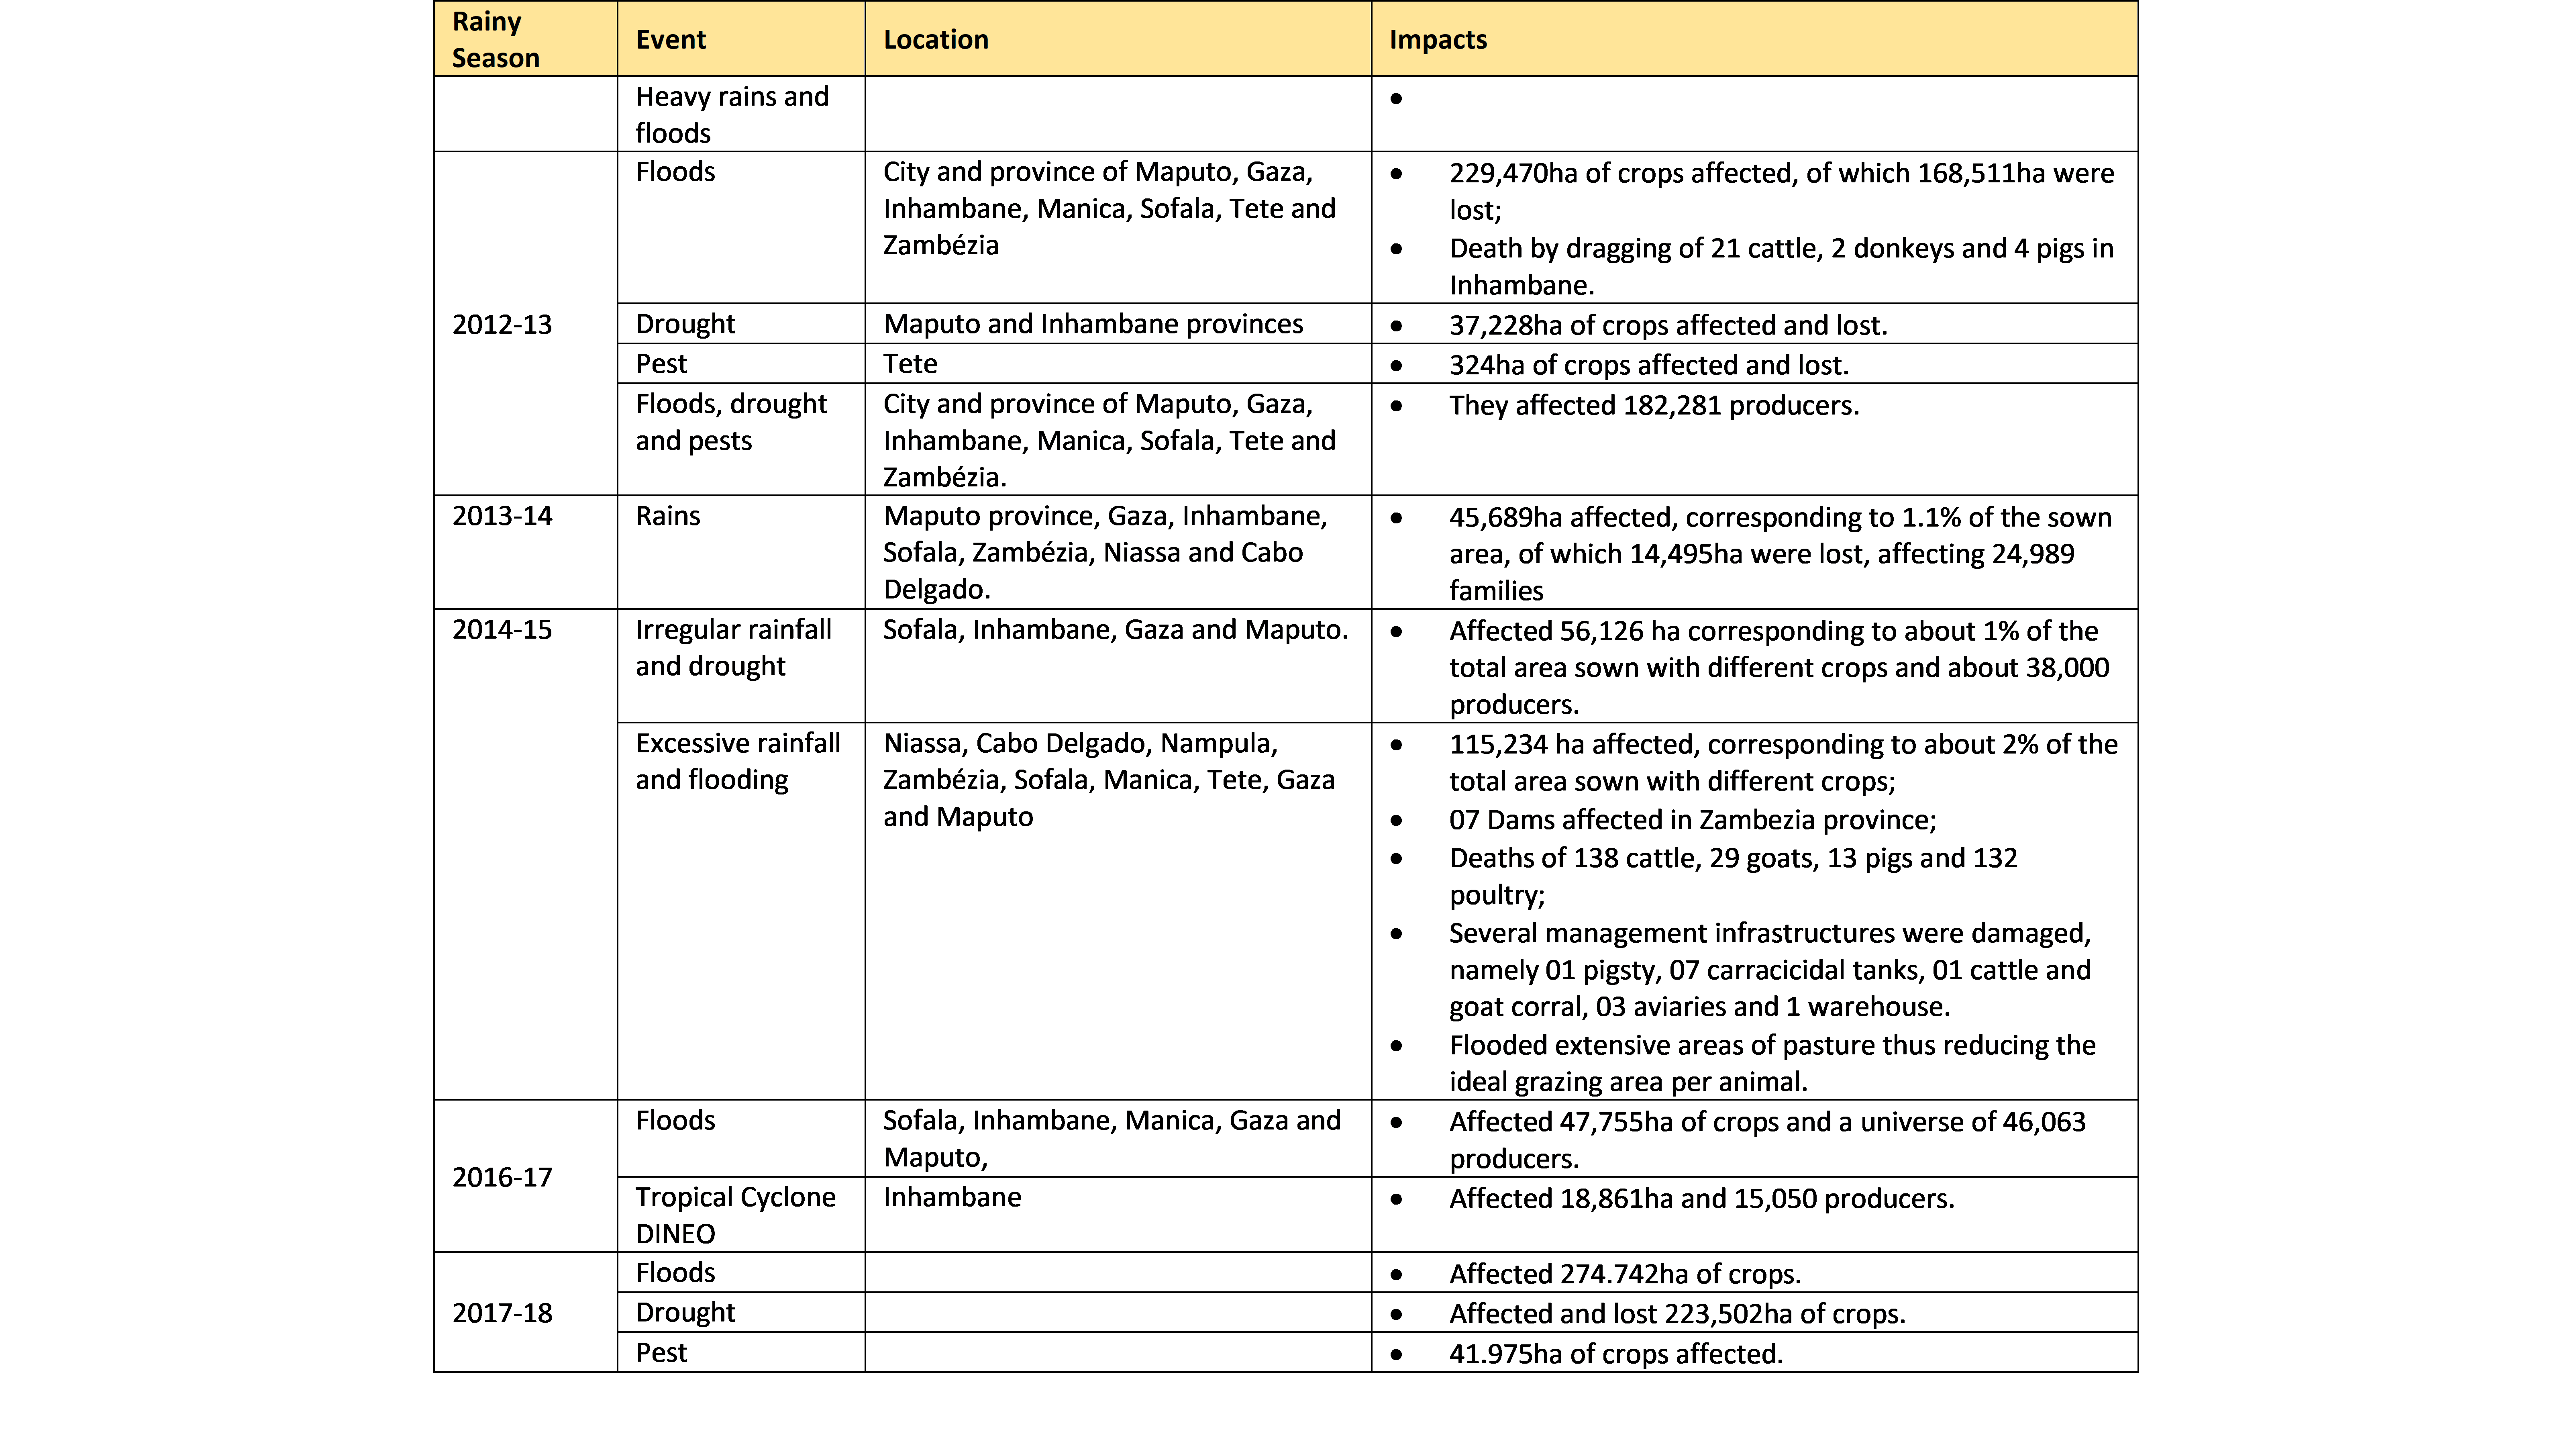
\includegraphics[width=1.5\textwidth,height=\textheight]{Agriculture-impact.png}

\emph{Source: Balances of the rainy seasons for the period 2011-12 to 2017-18}

Weather events in the country between the rainy seasons from 2011-12 to 2017-18 affected around 1,384,677 ha of crops, of which around 733,270 ha were lost. The events that affected the largest area of crops were the tropical depression Dando and the tropical cyclone Funso, which occurred in the 2011-12 rainy season, while the greatest loss of crops occurred following the floods of 2012-2013.

The events that cause most loss and destruction in the agricultural sector are those related to excessive rainfall and floods and tropical cyclones. However, when a drought occurs, usually the area affected equals the area lost.

It is also important to stress that in addition to the biophysical vulnerability associated with the occurrence of extreme weather events, the levels of technology adopted by most producers do not correspond to the requirements of the selected varieties, due to the weak financial capacity to purchase agricultural inputs, which also contributes to low production and productivity.

\textbf{\emph{Livestock}}

Livestock plays a vital role for the rural population, it is one of the components of agriculture. The contribution of livestock to the national economy is incipient. In 2008, livestock represented 10\% of total agricultural production and contributed only 1.7\% to the Gross Domestic Product (OIE Report, 2008). However, animal production is affected by climate change in food quantity and quality, disease distribution, management practices and production systems (Herrero et al.~2009).

The main constraints to the development of livestock production are as follows:

\begin{enumerate}
\def\labelenumi{(\roman{enumi})}
\item
  Low productivity of existing herds due to the genetic quality of breeding stock and inadequate management practices;
\item
  Weak veterinary assistance network for the family sector;
\item
  Lack of infrastructure for watering and managing livestock.
\end{enumerate}

PEDSA identifies drought as one of the environmental factors causing a notable loss of productivity and the use of technologies to improve water availability and management as a key element to improve livestock production. For example, in 2015, 6,767 cattle and 112 goats died nationwide due to drought.

In semi-arid regions, livestock production is a way for farmers to adapt to climate change, as animals are relatively less affected. However, several aspects of livestock production are affected by climate change, including feed quantity and quality, disease distribution, management practices and production systems (Herrero et al.~2009). Therefore, to achieve the above Government objectives, investment is needed to address any constraints to livestock productivity, including climate change.

The vulnerability and adaptation of pastures and livestock are matters of great concern in developing countries such as Mozambique, due to the great importance of livestock as a livelihood component and source of income for local communities. The objectives of this sub-chapter are:

\begin{enumerate}
\def\labelenumi{(\arabic{enumi})}
\item
  Assess the expected impacts and vulnerability of pasture and livestock to climate change;
\item
  Identify adaptation programmes and measures;
\item
  Identify gaps, needs and priorities for climate change education, training and public awareness.
\end{enumerate}

It should be noted that the impacts of extreme climate events on livestock are already a reality in the country, as illustrated in Table 3.4. The observed impacts range from the loss of animals through death to the destruction of livestock management infrastructures, including the loss of pasture areas.

\emph{Table 3.4: Impacts of extreme events on livestock}

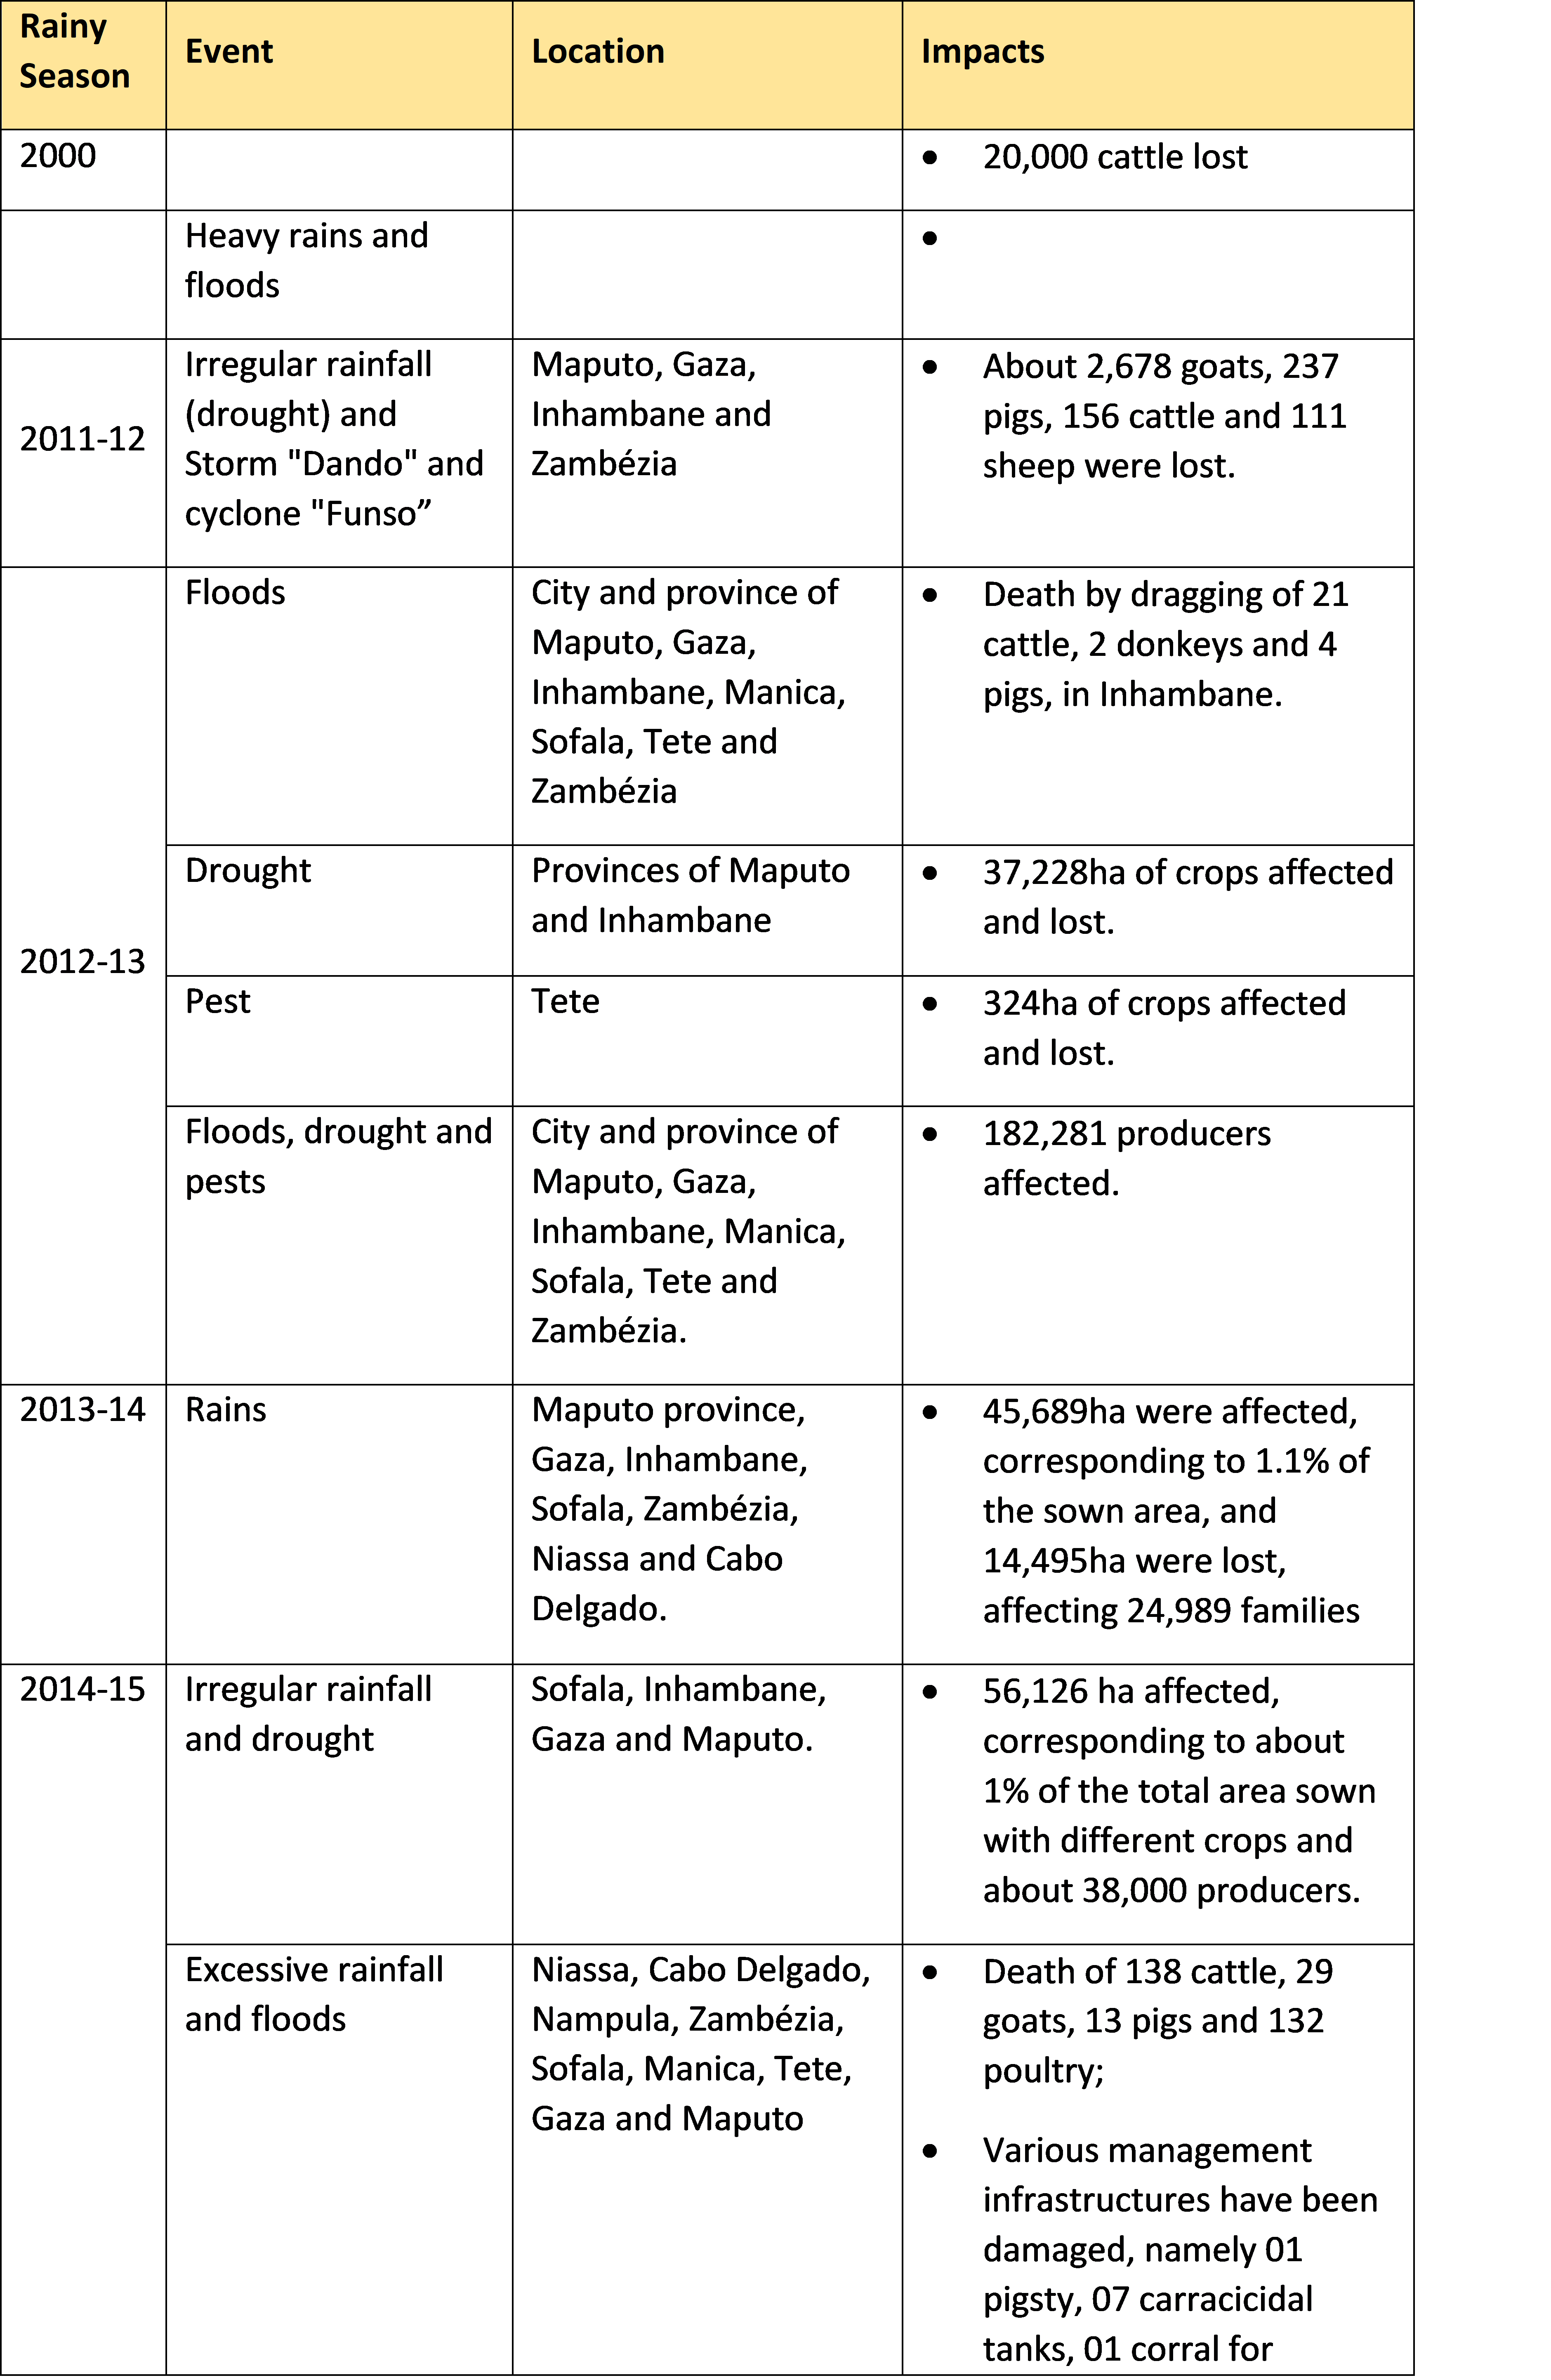
\includegraphics[width=0.75\textwidth,height=\textheight]{Livestock.png}

\hypertarget{fishery}{%
\section{Fishery}\label{fishery}}

\hypertarget{food-security-and-nutrition}{%
\section{Food Security and Nutrition}\label{food-security-and-nutrition}}

\hypertarget{water-resources}{%
\section{Water Resources}\label{water-resources}}

\hypertarget{health}{%
\section{Health}\label{health}}

\hypertarget{energy}{%
\section{Energy}\label{energy}}

\hypertarget{infrastructure}{%
\section{Infrastructure}\label{infrastructure}}

\hypertarget{coastal-zones}{%
\section{Coastal Zones}\label{coastal-zones}}

\hypertarget{disaster-risk-human-safety-and-wellbeing}{%
\section{Disaster risk: human safety and wellbeing}\label{disaster-risk-human-safety-and-wellbeing}}

\hypertarget{social-protection}{%
\section{Social Protection}\label{social-protection}}

\hypertarget{adaptation-priorities}{%
\chapter{Adaptation Priorities}\label{adaptation-priorities}}

\hypertarget{implementation-financing-me}{%
\chapter{Implementation, Financing, M\&E}\label{implementation-financing-me}}

\hypertarget{implementation-strategy}{%
\section{Implementation Strategy}\label{implementation-strategy}}

\hypertarget{financial-resources}{%
\section{Financial Resources}\label{financial-resources}}

\hypertarget{me-and-reporting}{%
\section{M\&E and Reporting}\label{me-and-reporting}}

\hypertarget{annexes}{%
\chapter{Annexes}\label{annexes}}

  \bibliography{book.bib,packages.bib}

\end{document}
